\section{Fase 7: Evaluación e Interpretación}
En esta fase, el \textit{Data Analysis Team} evalúa el modelo para comprender su calidad y garantizar que este aborda las preguntas generadas en el \textit{BCQM} de manera adecuada y completa. Es necesario que para realizar la evaluación se utilicen medidas especializadas basadas en el rendimiento, sensibilidad y especificidad del modelo. Adicionalmente, los resultados obtenidos deben ser entendibles por el medico experto en oncología, en donde se garantice que dichos resultados sean interpretados correctamente y estén relacionados a la estadificación y los biomarcadores del cáncer de mama. Es importante que el medico junto al científico de datos ajusten el modelo según las necesidades. Dado que se esta trabajando con datos médicos sensibles, es necesario que al modelo final se aplique a un conjunto de validación para realizar una evaluación final. Además, el \textit{Data Analysis Team} puede asignar al modelo pruebas de \textit{significancia estadística} como prueba adicional para comprobar la respuesta obtenida a la pregunta generada. Esta prueba adicional es fundamental para justificar la implementación del modelo. Finalmente, dado que en el \textit{BCQM} se pueden plantear múltiples preguntas relacionadas a diferentes tipo de cáncer de mama y técnicas de diagnostico durante el \textit{Release}, es necesario que los científicos con ayuda del ingeniero de datos unan, si es posible, los resultados obtenidos en una matriz o mapa de calor para identificar el coeficiente de correlación entre dos o mas variables oncológicas. Esta matriz resultante debe ser analizada por el medico experto en oncología para determinar si existe una relación significativa entre los diferentes tipos de cáncer de mama.

Con base a los resultados obtenidos en la fase anterior, el modelo \textit{BIRCH} fue el seleccionado para agrupar los datos genómicos del conjunto de datos del carcinoma invasivo de mama (TCGA, Cell 2015) en \textit{clusters} basados en los tipos de cáncer lobulillar invasivo(LBC), ductal invasivo(IDC) o de tumores mixtos(MTBC).

\subsection{Agrupamiento BIRCH}
El  método de agrupación de datos \textit{BIRCH}(Balanced, Iterative Reducing , and Clustering using Hierarchies) reúne de forma incremental y dinámica puntos de datos métricos multidimensionales entrantes para intentar producir una agrupación de mejor calidad con los recursos disponibles, es decir, la memoria disponible y las limitaciones de tiempo. Por lo general, BIRCH puede encontrar una buena agrupación con una sola exploración de los datos y mejorar aún más la calidad con unas pocas exploraciones adicionales. BIRCH es también el primer algoritmo de clustering propuesto en el área de bases de datos que maneja eficazmente el \textit{“ruido”}, es decir puntos de datos que no forman parte del patrón subyacente \cite{Zhang1996}. 

Este modelo, presentó un mayor desempeño al medir la eficiencia espacio-temporal, la sensibilidad al orden de entrada de los datos y la calidad de la agrupación mediante varias iteraciones. El resultado obtenido puede ser observado en la figura \ref{BIRCH_TSNE} generada con el método T-SNE que permite visualizar las similitudes entre vecinos en un espacio multidimensional y  la figura \ref{BIRCH_PCA} que permite visualizar la distancia entre clusters según el análisis de componentes principales (PCA\footnote{PCA: Principal Component Analysis}). Dado lo anterior, en la gráficas se visualiza que los clusters presentan una metrica de cohesión y separación que permite identificar las 4 agrupaciones generadas por el modelo BIRCH .

\begin{figure}
	\centering
	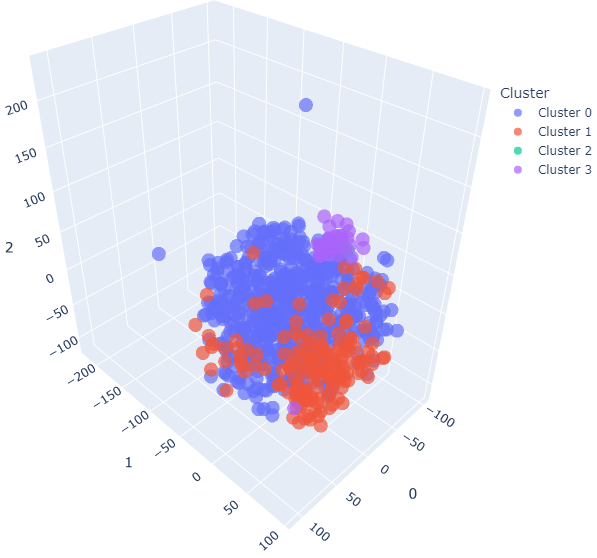
\includegraphics[width=0.5
	\linewidth]{NOTEBOOK/IMAGENES_CLUSTERING/8_TNSE_Birch_Clustering}
	\caption{T-SNE generado por el modelo BIRCH.}
	\label{BIRCH_TSNE}
\end{figure}

\begin{figure}
	\centering
	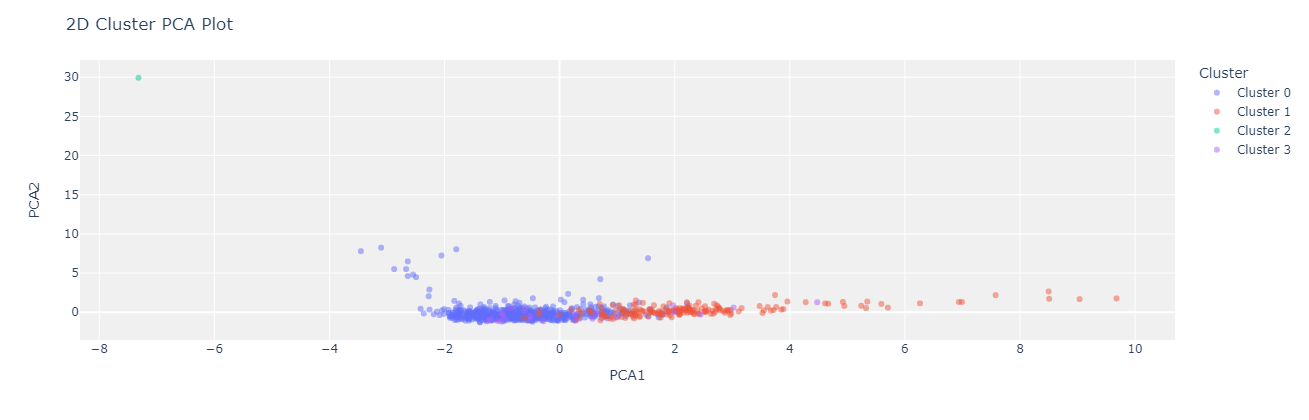
\includegraphics[width=1
	\linewidth]{NOTEBOOK/IMAGENES_CLUSTERING/8_PCA_Birch_Clustering}
	\caption{PCA generado por el modelo BIRCH.}
	\label{BIRCH_PCA}
\end{figure}

\subsection{Métricas para la validación del Clustering}
Como se afirmo anteriormente, en esta fase se realizó la evaluación de los resultados obtenidos por el modelo \textit{BIRCH}. Conviene subrayar, que la validación externa y la validación interna son las dos categorías más importantes para la validación de los modelos de agrupamiento. La principal diferencia es si se usa o no información externa para la validación, es decir, información que no es producto de la técnica de agrupación utilizada\cite{Elizabeth2023}. Dada la naturaleza del algoritmo y de lo datos, en este caso se utilizo \textit{validación interna} para medir el clustering generado por el modelo BIRCH únicamente basados en información de los datos del carcinoma invasivo de mama (TCGA, Cell 2015), lo cual nos permitió evaluar que tan buena fue la estructura del clustering sin necesidad de información ajena al propio algoritmo y su resultado. Como el objetivo del clustering es agrupar objetos similares en el mismo clúster y objetos diferentes ubicarlos en diferentes clúster, las métricas de validación interna están basadas usualmente en los dos siguientes criterios\cite{Elizabeth2023}:
\begin{itemize}[label=\HandRight]
	\item \textbf{Cohesión}: El miembro de cada clúster debe ser lo más cercano posible a los otros miembros del mismo clúster.
	\item \textbf{Separación}: Los clúster deben estar ampliamente separados entre ellos.
\end{itemize}
Dado lo anterior, se seleccionaron las siguientes métricas de validación internas:
%-------------------------------------------
\subsubsection{Indice de Davies-Bouldien}
Este indice representa el promedio de las distancias que pertenecen a un determinado cluster.	Valores pequeños para el índice $DB$ indica clústeres compactos, y cuyos centros están bien separados los unos de los otros. Consecuentemente el número de clústeres que minimiza el índice Davies-Bouldien se toma como el óptimo. Dado lo anterior, este indice esta definido como:
\begin{equation}
	DB = \frac{1}{k} \sum_{i=1,i\neq j}^{k} max \left( \frac{\sigma_{i}+\sigma_{j}}{d(c_{i},c_{j})}\right) 
\end{equation}
\begin{itemize}[label=]
	\item $k=$ número de clústeres.
	\item $\sigma_{i}=$ distancia promedio entre cada punto en el clúster $i$ y el centroide del clúster.
	\item $\sigma_{j}=$ distancia promedio entre cada punto en el clúster $j$ y el centroide del clúster.
	\item $d(c_{i},c_{j})=$ distancia entre los centroides de los 2 clústeres .
\end{itemize}
%-------------------------------------------
\subsubsection{Coeficiente de silhouette} 
Esta metrica permite identificar cual es el numero optimo de agrupamientos. Dado lo anterior, esta definido como:
\begin{itemize}[label=]
		\item $a(x)=$ distancia promedio de $x$ a todos los demás puntos en el mismo cluster.
		\item $b(x)=$ distancia promedio de $x$ a todos los demás puntos en el cluster más cercano.
\end{itemize}
Dado esto, se dice que el coeficiente de la silueta para $x$ está dado por:
\begin{equation}
	s(x) = \frac{b(x)-a(x)}{max\left\lbrace a(x), b(x) \right\rbrace }
\end{equation}

Donde el valor de $s(x)$ puede variar entre $-1$ y $1$. En donde, $-1$ es interpretado como un mal agrupamiento, $0$ como un resultado indiferente y $1$ como un buen agrupamiento \cite{Ramirez2018}. Por lo tanto, el coeficiente de la silueta para todo el agrupamiento es:
	
\begin{equation}
	SC = \frac{1}{N} \sum_{i = 1}^{N}s(x)
\end{equation}
%-------------------------------------------
\subsubsection{Método del codo}
Esta metrica utiliza los valores de la inercia obtenidos tras aplicar el algoritmo de agrupamiento a diferente número de clusters (desde $1$ a $N$ clusters), siendo la inercia la suma de las distancias al cuadrado de cada objeto del cluster a su centroide:
	
\begin{equation}
	inercia = \sum_{i = 0}^{N}  \parallel x_{i} - \mu  \parallel
\end{equation}
	
Una vez obtenidos los valores, se representa en una gráfica lineal la inercia respecto del número de clusters. En esta gráfica se debería apreciar un cambio brusco en la evolución de la inercia, teniendo la línea representada una forma similar a la de un brazo y su codo. El punto en el que se observa ese cambio nos indica el número óptimo de clusters a seleccionar para el conjunto de datos en cuestión \cite{Moya2022}. 

%-------------------------------------------
\subsection{Evaluación del modelo BIRCH}
Con base a las métricas de validación internas aplicadas al modelo BIRCH, se obtuvo un indice de Davies-Bouldien del $1.8703$, valor que ratifica que lo centros están separados correctamente, tal y como se observa en la tabla \ref{Davies-Bouldien}. Adicionalmente, en la figura \ref{a} se observan los 4 clusters generados por el modelo para un coeficiente de Silhouette del $0.1286$. Por ultimo, en la figura \ref{b} se observa que la inercia se produce en $k = 5 $, corroborando el resultado del coeficiente de Silhouette obtenido anteriormente y confirmando que el modelo tiene el numero de clusters adecuado. Por consiguiente se infiere que el modelo presenta clústeres compactos con centros considerablemente separados los unos de los otros lo cual indica que el agrupamiento generado para el conjunto de datos del carcinoma invasivo de mama es aceptable. 

\begin{table*}[!htb]
	\footnotesize
	\centering
	\begin{threeparttable}
		\begin{tabular}{p{1cm} p{4cm} p{2.5cm} p{2.5cm} p{1.5cm}} \toprule	
			\begin{center}Id\end{center}
			&\begin{center}Modelo Clustering\end{center}
			&\begin{center}Silhouette\end{center}
			&\begin{center}Davies-Bouldin\end{center}
			&\begin{center}Clusters\end{center}
			\\ \hline 8 & BIRCH Clustering	&	0,1286	&	1,8703	&	4
			\\ \hline
		\end{tabular}
		\caption{Indice de Davies-Bouldien del modelo BIRCH.}
		\label{Davies-Bouldien}
	\end{threeparttable}
\end{table*}

\begin{figure}[!htb]
	\centering
	\subfloat[Coeficiente de Silhouette]{\label{a}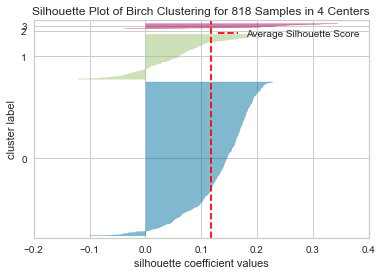
\includegraphics[width=0.5\linewidth]{NOTEBOOK/IMAGENES_CLUSTERING/8_SILHOUTETTE_Birch_Clustering}}\hfill
	\subfloat[Método del codo]{\label{b}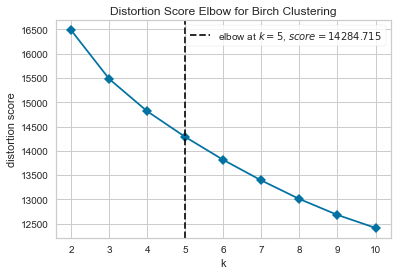
\includegraphics[width=0.5\linewidth]{NOTEBOOK/IMAGENES_CLUSTERING/8_ELBOW_Birch_Clustering}}\par 
	\caption{Métricas de validación internas modelo de agrupamiento BIRCH}
	\label{Silhouette_Elbow}
\end{figure}

\clearpage
%-------------------------------------------
\subsection{Interpretación de los resultados}
Con base a los 4 \textit{clusters} generados por el modelo \textit{BIRCH}, se procedió a identificar las características de origen genómico compartidas por 818 pacientes para analizar su comportamiento y así dar respuesta a las preguntas generadas en el BCQM. Dado lo anterior, se genero un análisis diagnostico para determinar las causas de las tendencias y las correlaciones de dichas variables con los tipos de cáncer de mama Lobulillar Invasivo (LBC), Ductal Invasivo (IDC) y Tumores Mixtos (MTBC). Se debe agregar que los clusters están conformados por 41 variables distribuidas en 9 variables numéricas y 33 variables categóricas, en donde el \textit{Cluster 0} agrupo 615 pacientes, el \textit{Cluster 1} agrupo 180 pacientes, el \textit{Cluster 2} agrupo 1 paciente y el \textit{Cluster 3} agrupo 22 pacientes. Los detalles de lo agrupación de los clusters por variable se pueden observar en la tabla \ref{clusters}:
\begin{table}[!htb]
	\begin{center} 
		\begin{tabular}{ |c|c|c|c| }
         \hline 
         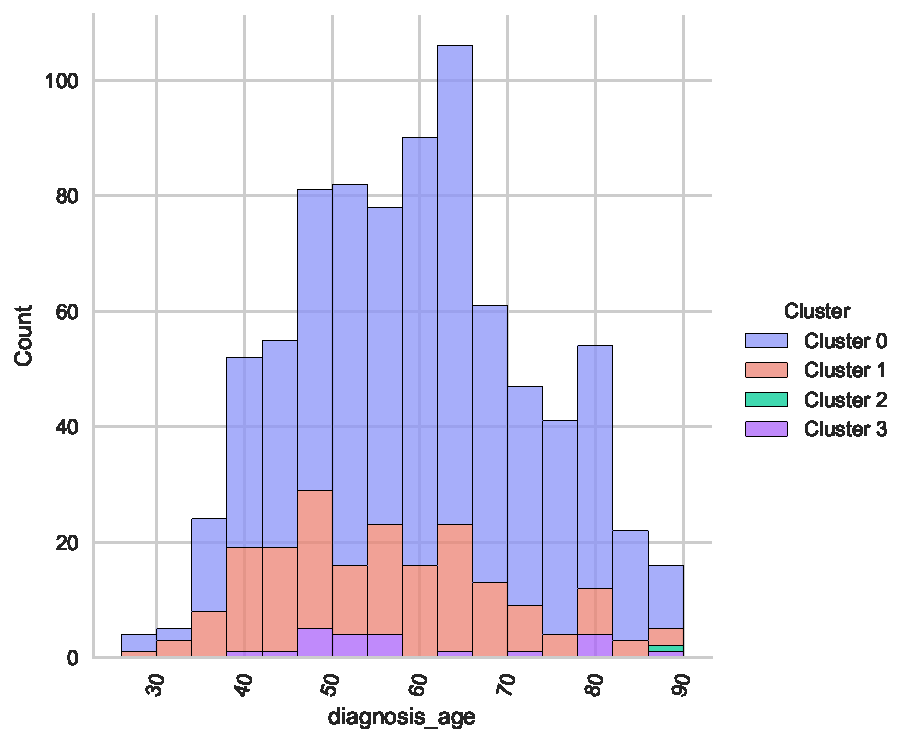
\includegraphics[width=0.21\textwidth]{NOTEBOOK/IMAGENES_BIRCH_DESCRIPTIVAS/1} 
         & 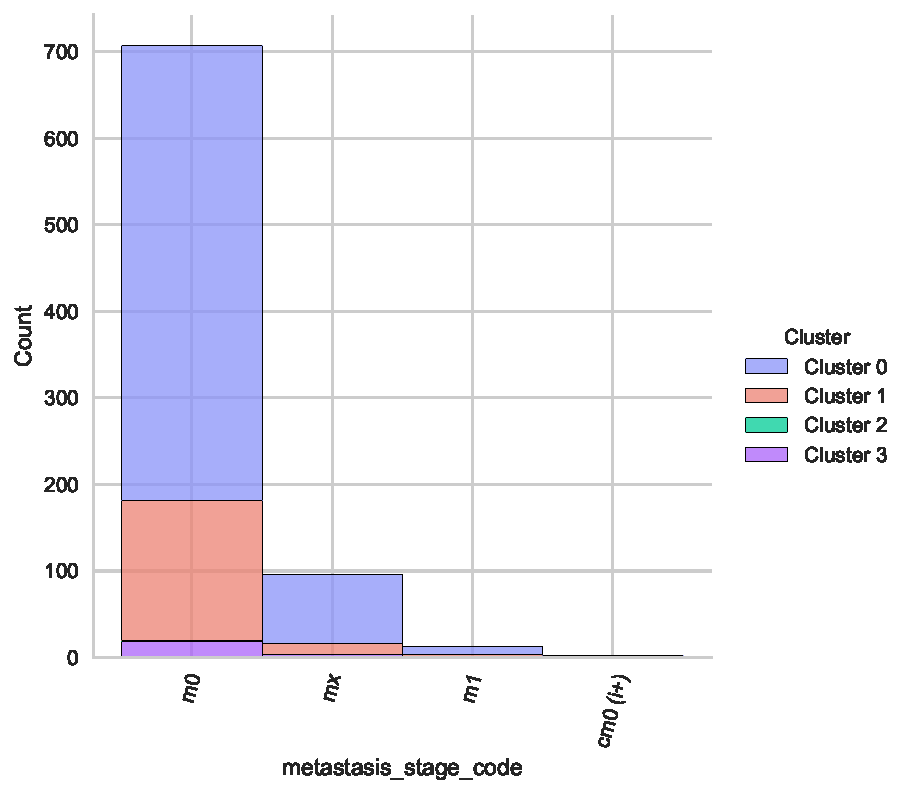
\includegraphics[width=0.21\textwidth]{NOTEBOOK/IMAGENES_BIRCH_DESCRIPTIVAS/2} 
         & 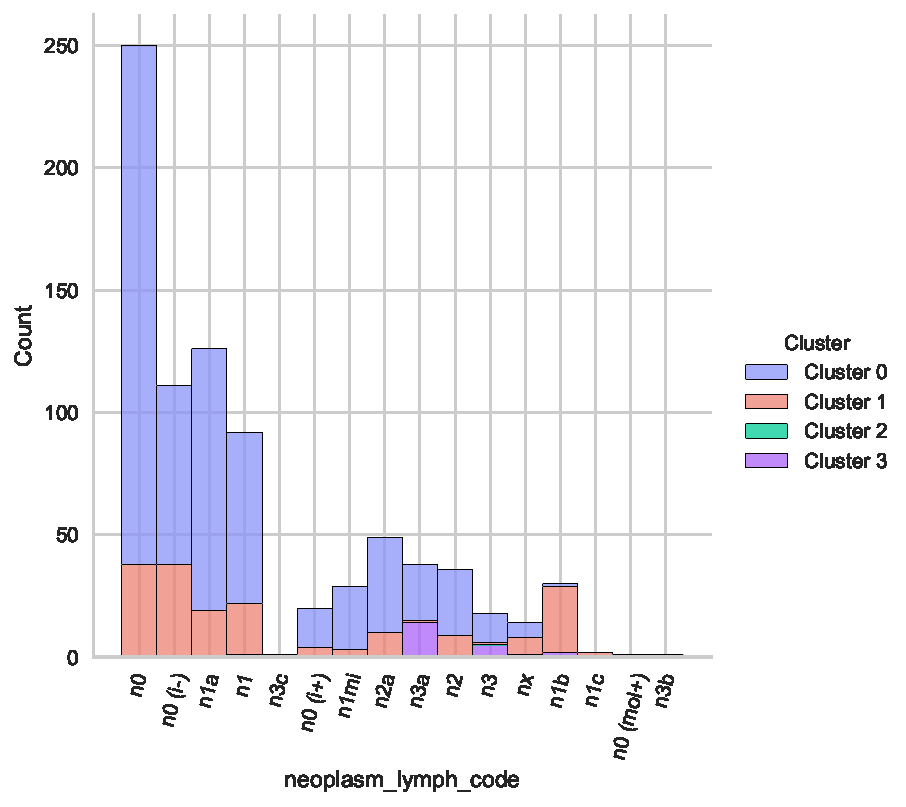
\includegraphics[width=0.21\textwidth]{NOTEBOOK/IMAGENES_BIRCH_DESCRIPTIVAS/3}
         & 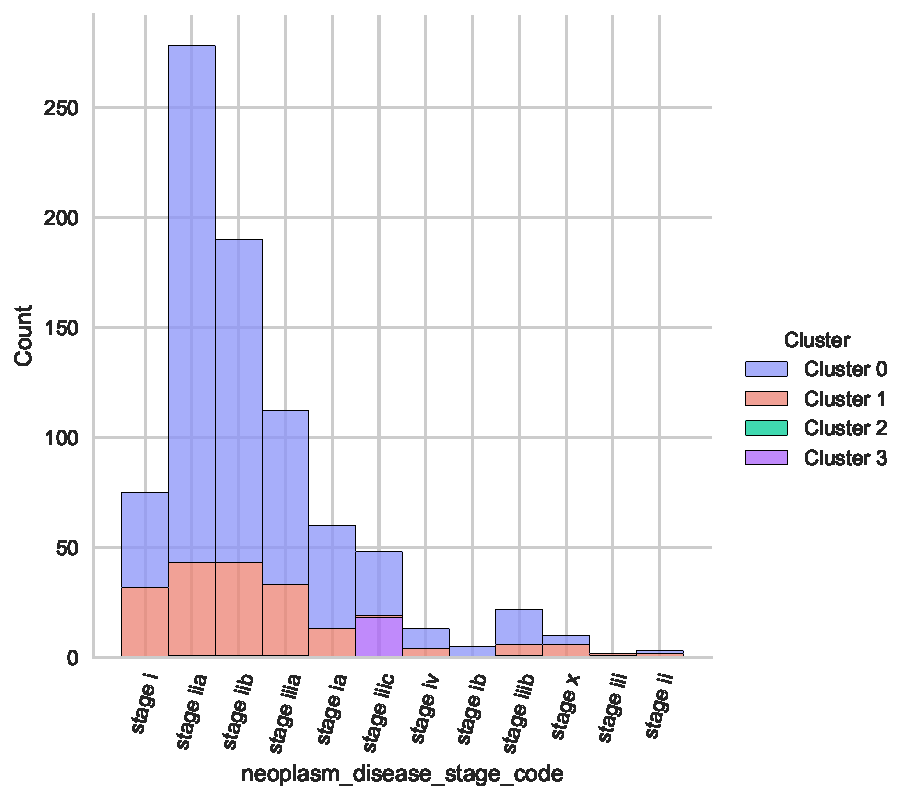
\includegraphics[width=0.21\textwidth]{NOTEBOOK/IMAGENES_BIRCH_DESCRIPTIVAS/4} 
         \\  \hline 
         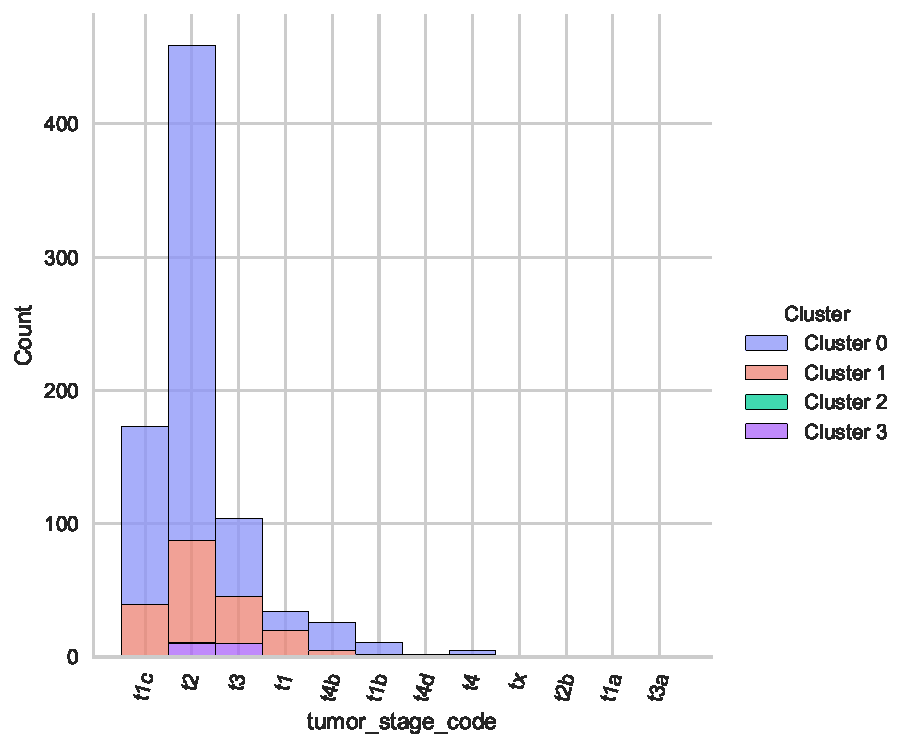
\includegraphics[width=0.21\textwidth]{NOTEBOOK/IMAGENES_BIRCH_DESCRIPTIVAS/5} 
         & 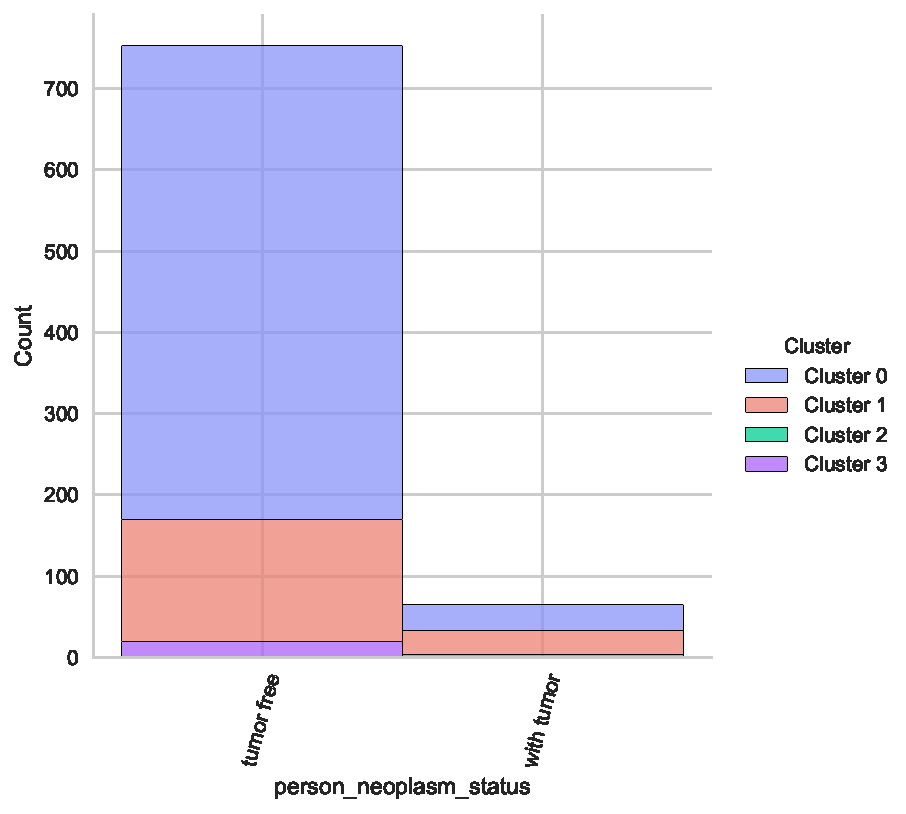
\includegraphics[width=0.21\textwidth]{NOTEBOOK/IMAGENES_BIRCH_DESCRIPTIVAS/41} 
         & 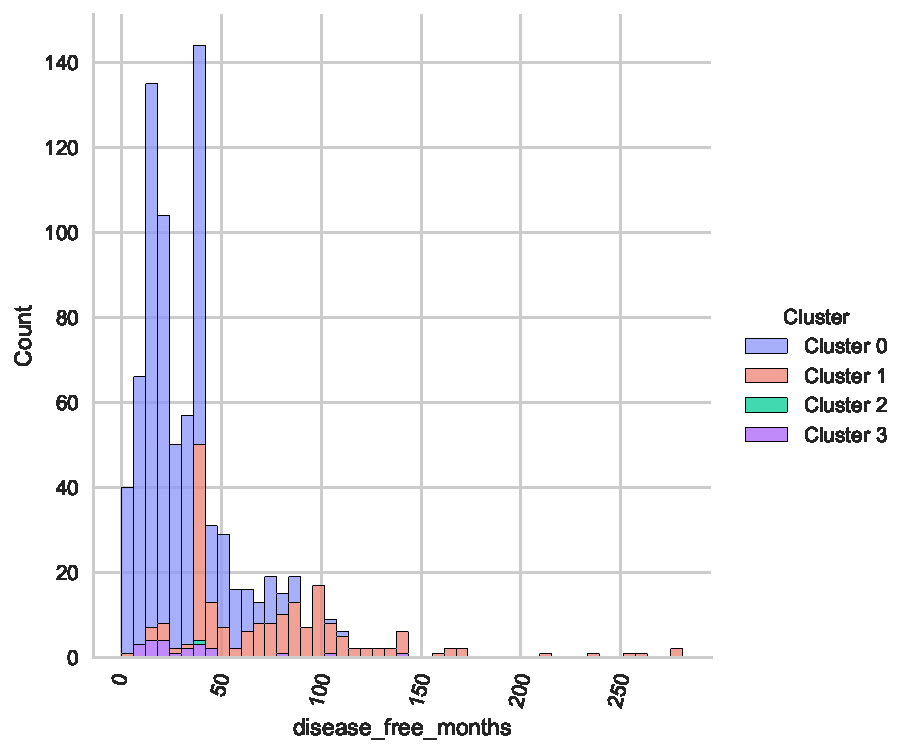
\includegraphics[width=0.21\textwidth]{NOTEBOOK/IMAGENES_BIRCH_DESCRIPTIVAS/7} 
         & 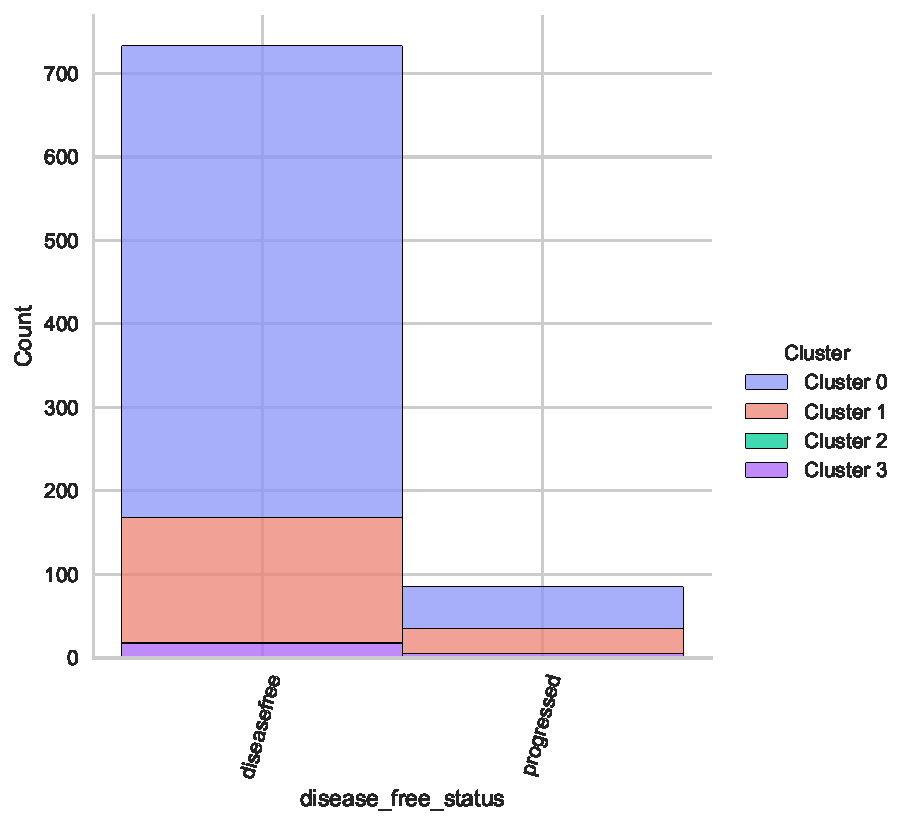
\includegraphics[width=0.21\textwidth]{NOTEBOOK/IMAGENES_BIRCH_DESCRIPTIVAS/8} 
         \\  \hline 
         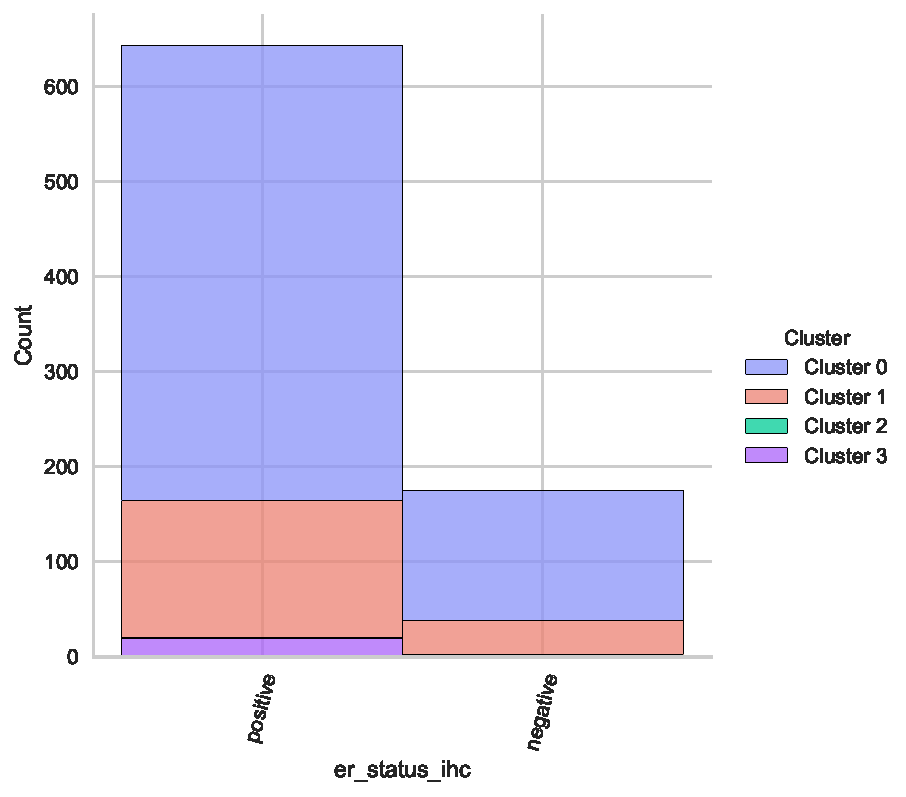
\includegraphics[width=0.21\textwidth]{NOTEBOOK/IMAGENES_BIRCH_DESCRIPTIVAS/9} 
         & 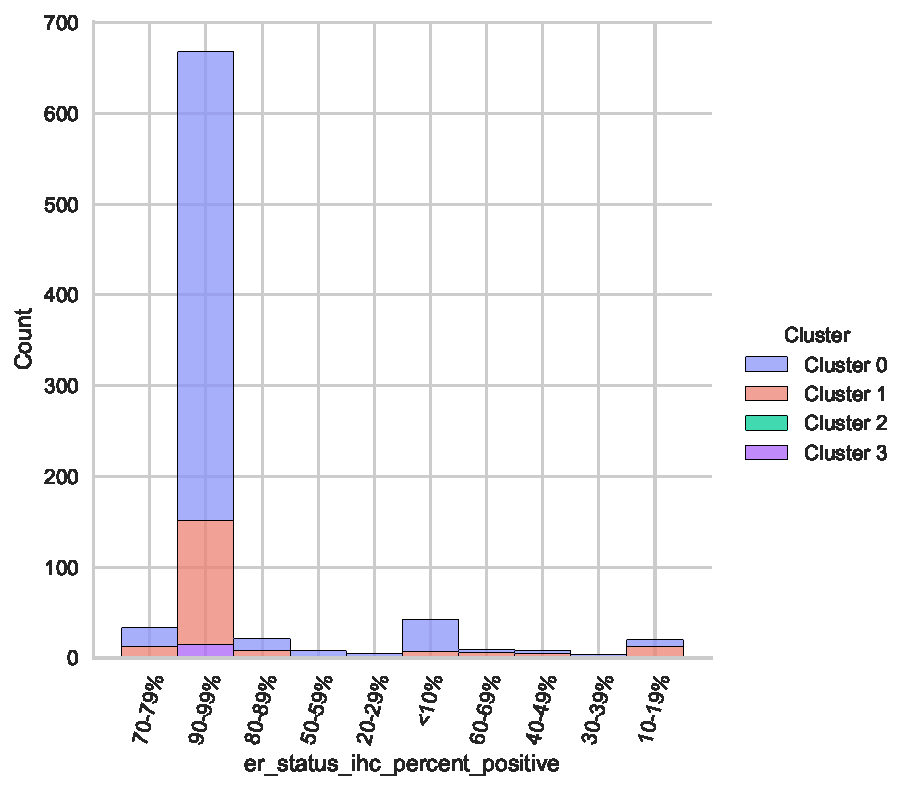
\includegraphics[width=0.21\textwidth]{NOTEBOOK/IMAGENES_BIRCH_DESCRIPTIVAS/10} 
         & 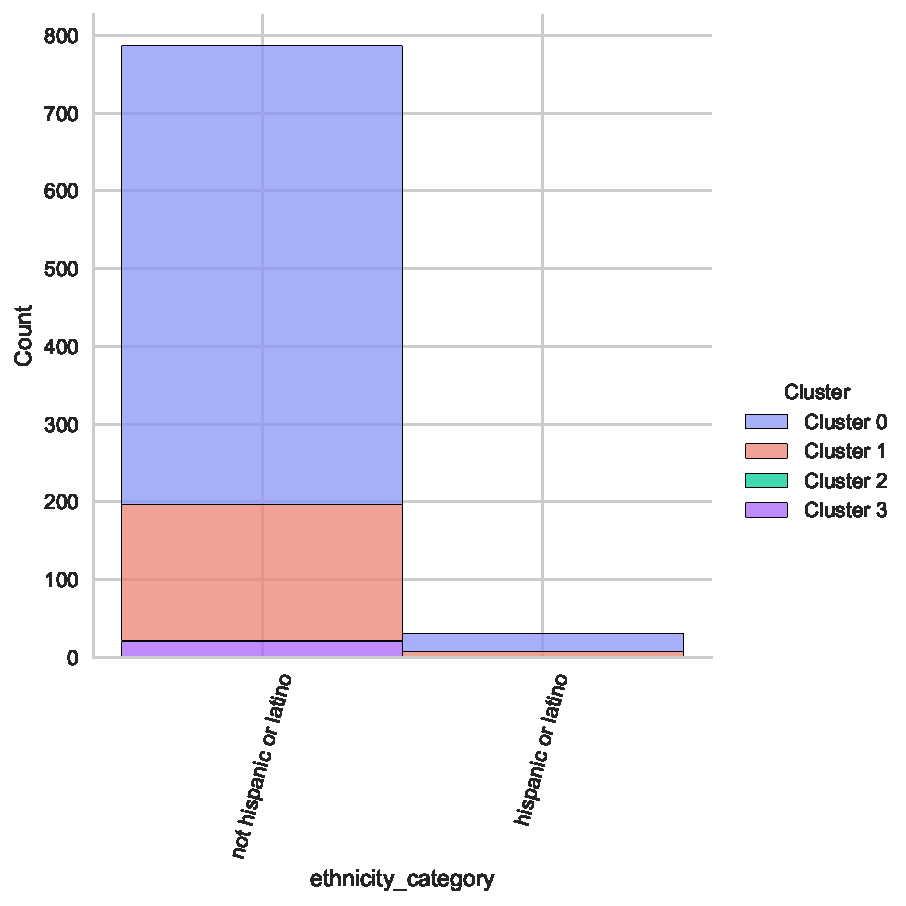
\includegraphics[width=0.21\textwidth]{NOTEBOOK/IMAGENES_BIRCH_DESCRIPTIVAS/11} 
         & 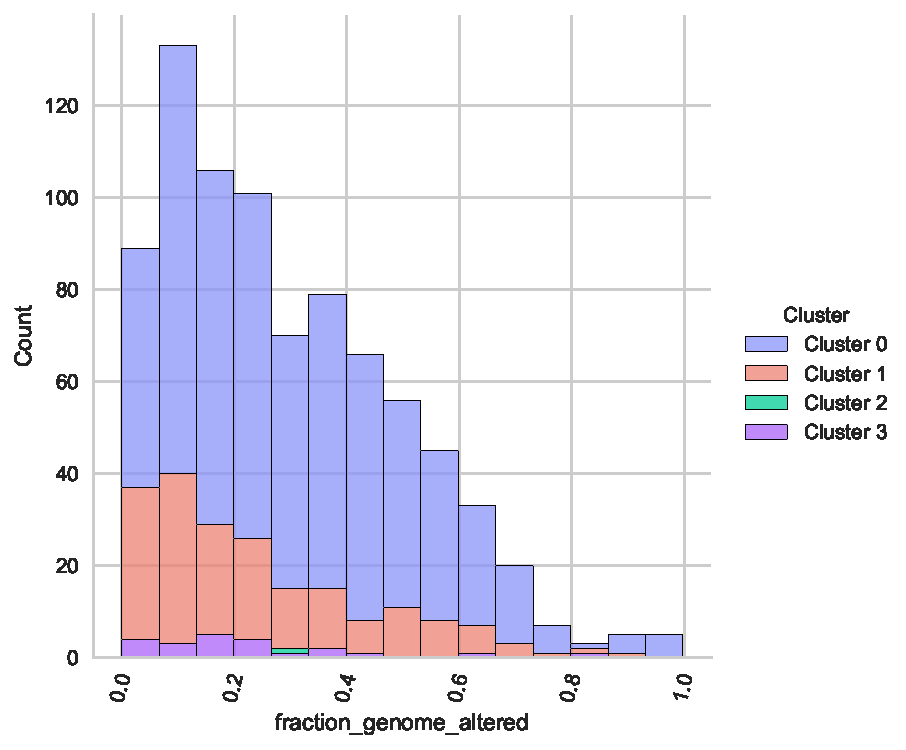
\includegraphics[width=0.21\textwidth]{NOTEBOOK/IMAGENES_BIRCH_DESCRIPTIVAS/12} 
         \\  \hline 
         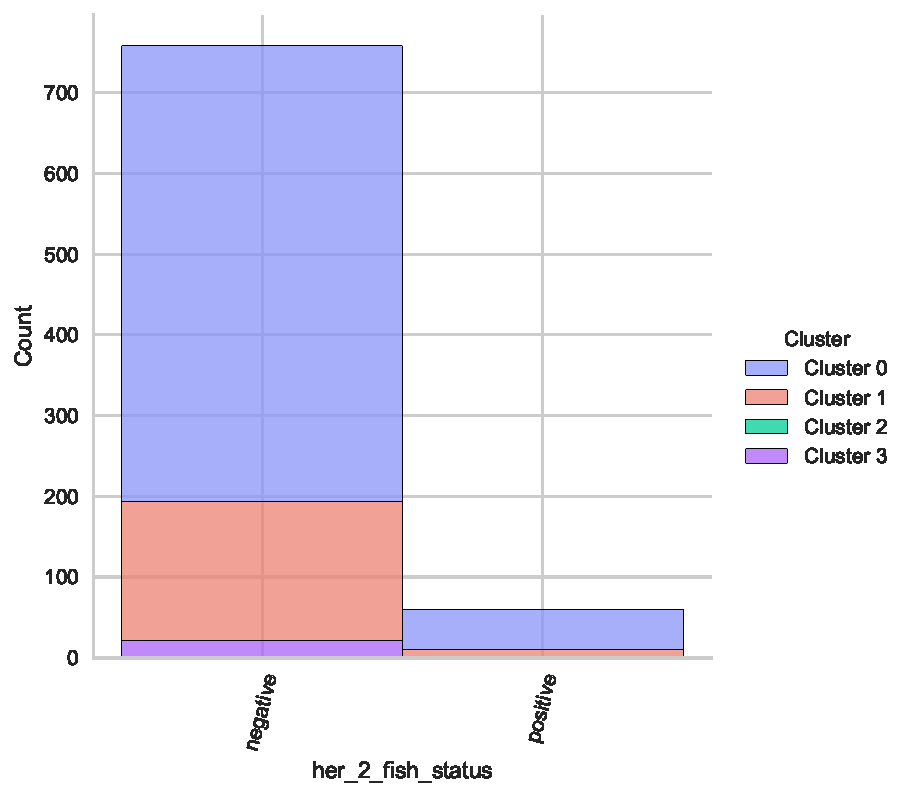
\includegraphics[width=0.21\textwidth]{NOTEBOOK/IMAGENES_BIRCH_DESCRIPTIVAS/13} 
         & 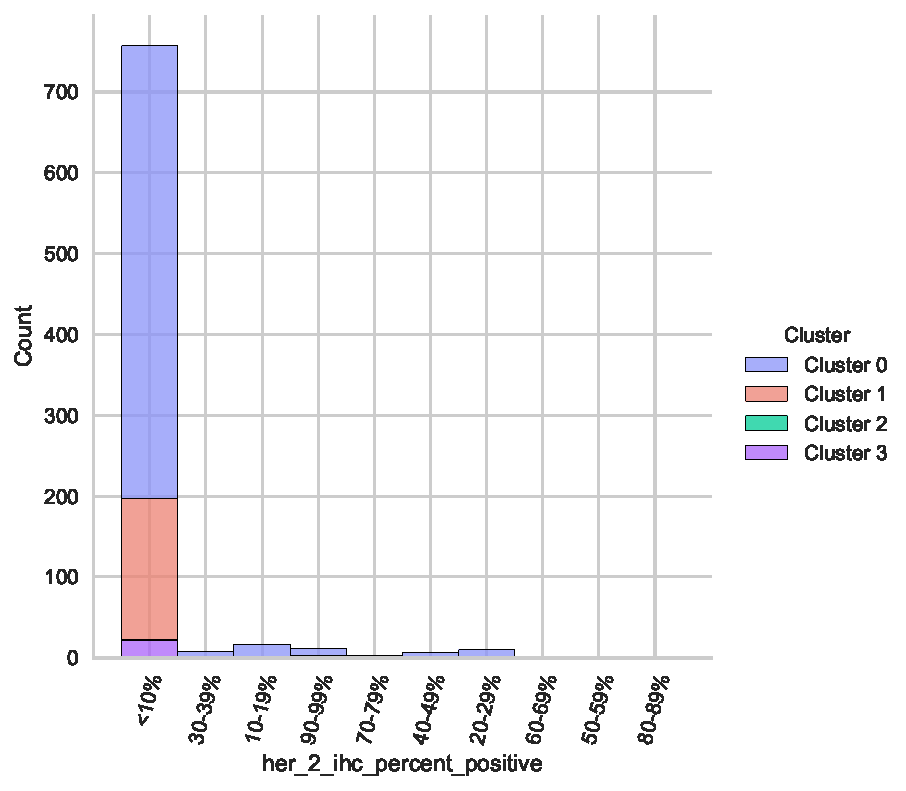
\includegraphics[width=0.21\textwidth]{NOTEBOOK/IMAGENES_BIRCH_DESCRIPTIVAS/14} 
         & 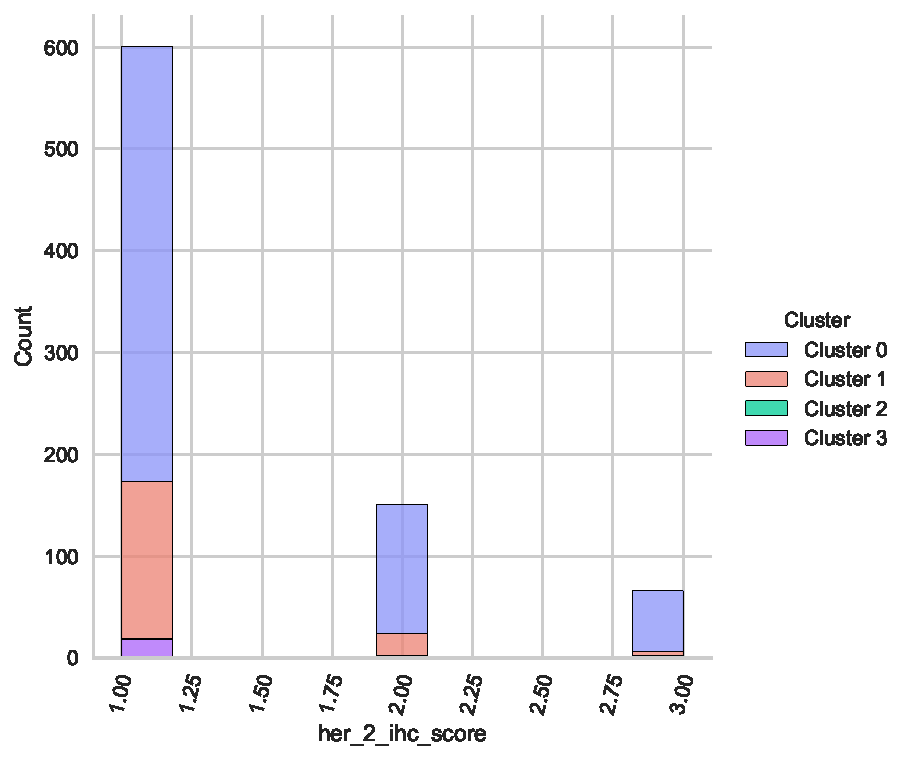
\includegraphics[width=0.21\textwidth]{NOTEBOOK/IMAGENES_BIRCH_DESCRIPTIVAS/15} 
         & 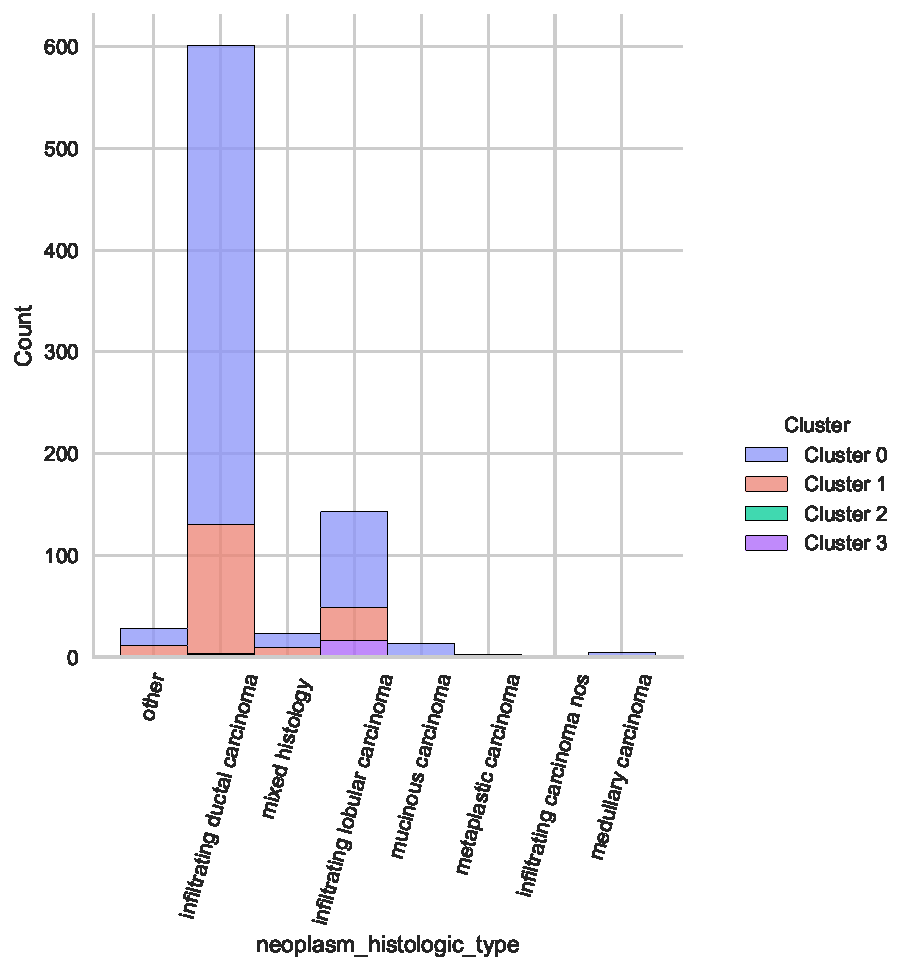
\includegraphics[width=0.21\textwidth]{NOTEBOOK/IMAGENES_BIRCH_DESCRIPTIVAS/16} 
         \\  \hline    
		\end{tabular} 
	\end{center} 
\end{table}

\begin{table}
	\begin{center} 
		\begin{tabular}{ |c|c|c|c| }
			\hline 
			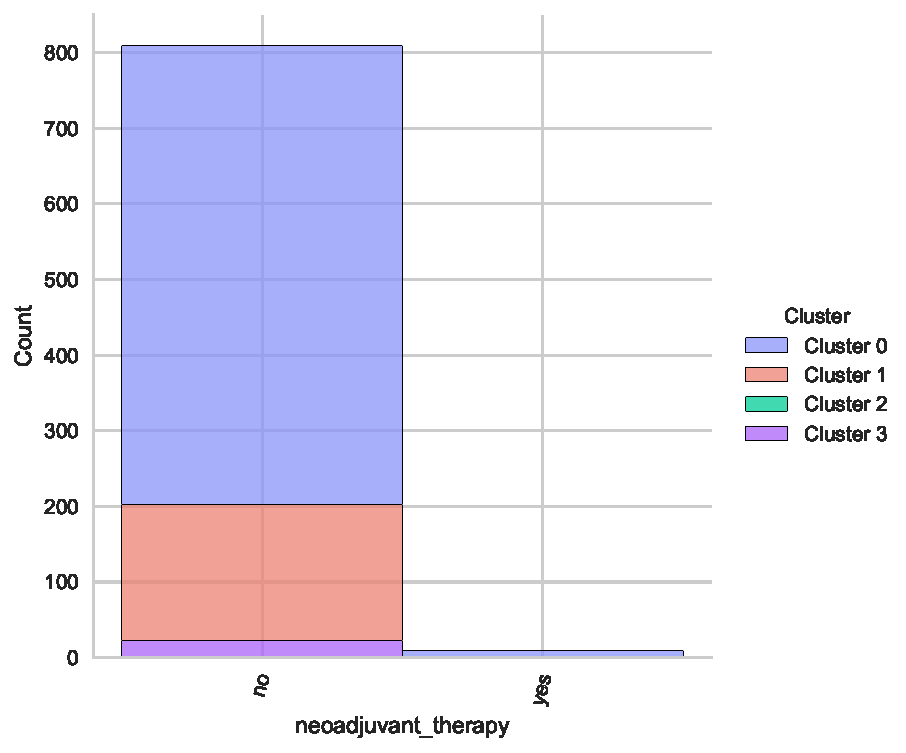
\includegraphics[width=0.22\textwidth]{NOTEBOOK/IMAGENES_BIRCH_DESCRIPTIVAS/17} 
			& 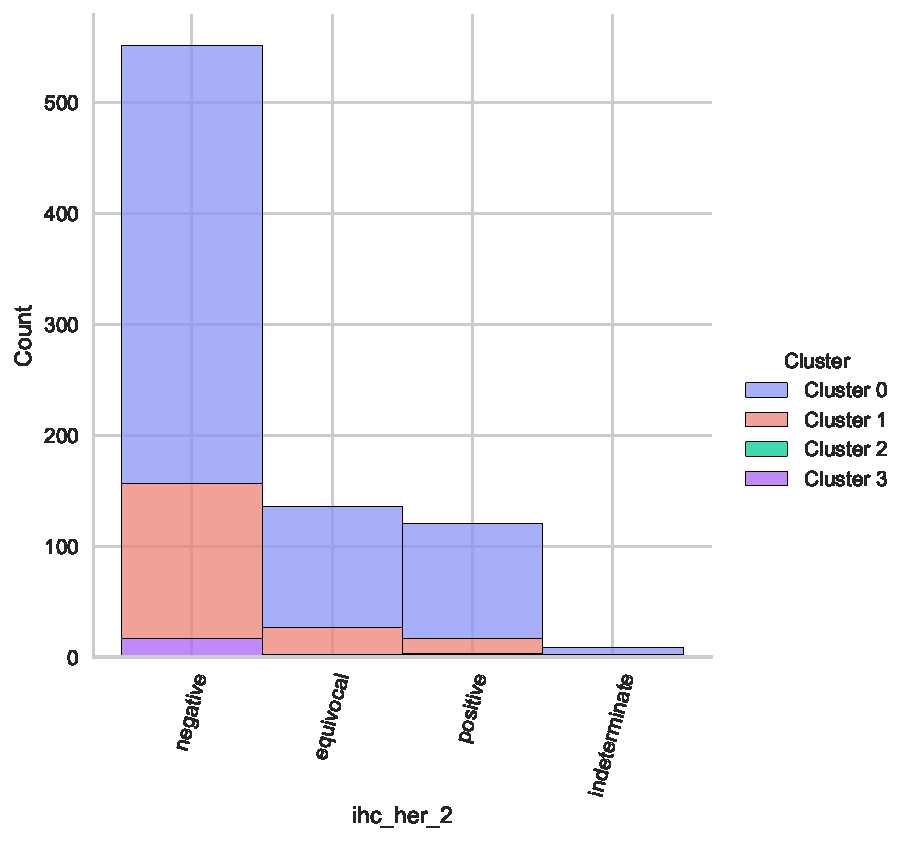
\includegraphics[width=0.22\textwidth]{NOTEBOOK/IMAGENES_BIRCH_DESCRIPTIVAS/18} 
			& 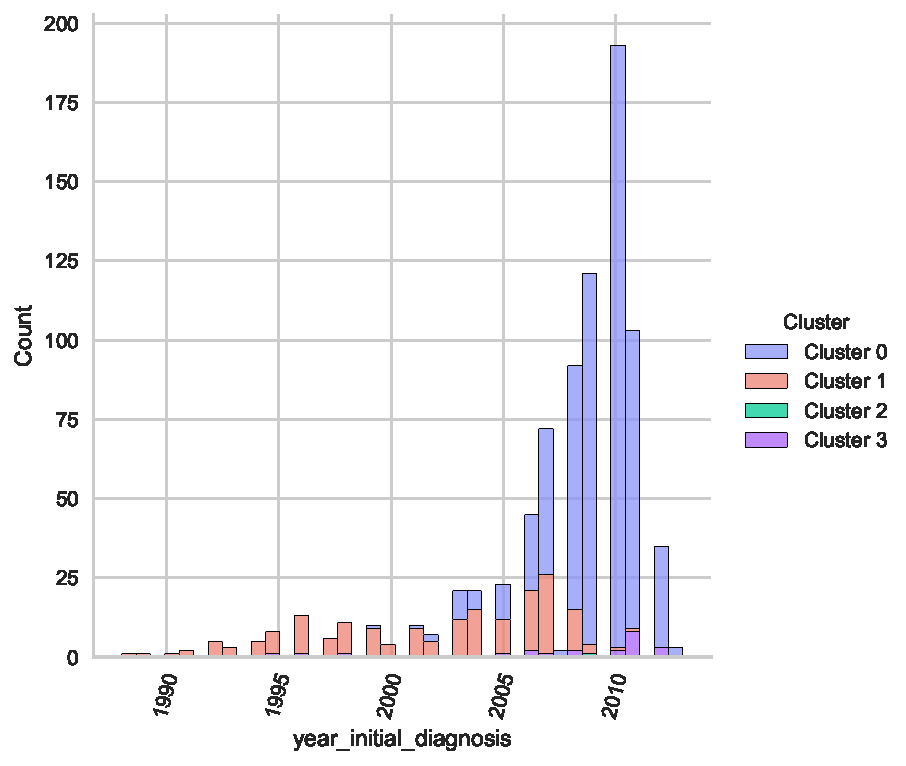
\includegraphics[width=0.22\textwidth]{NOTEBOOK/IMAGENES_BIRCH_DESCRIPTIVAS/19} 
			& 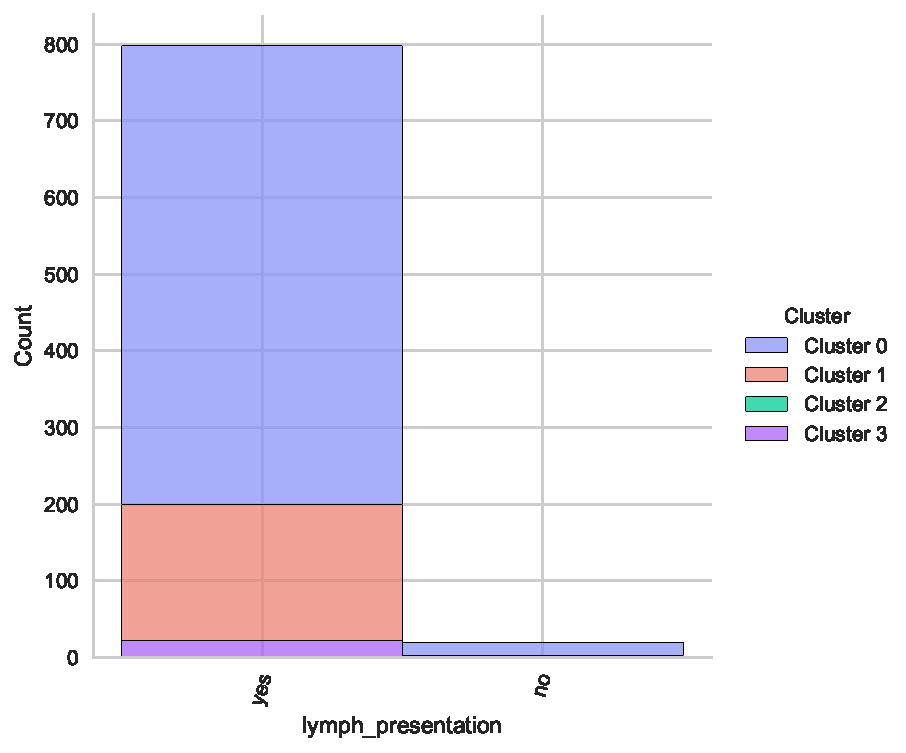
\includegraphics[width=0.22\textwidth]{NOTEBOOK/IMAGENES_BIRCH_DESCRIPTIVAS/20} 
			\\  \hline
			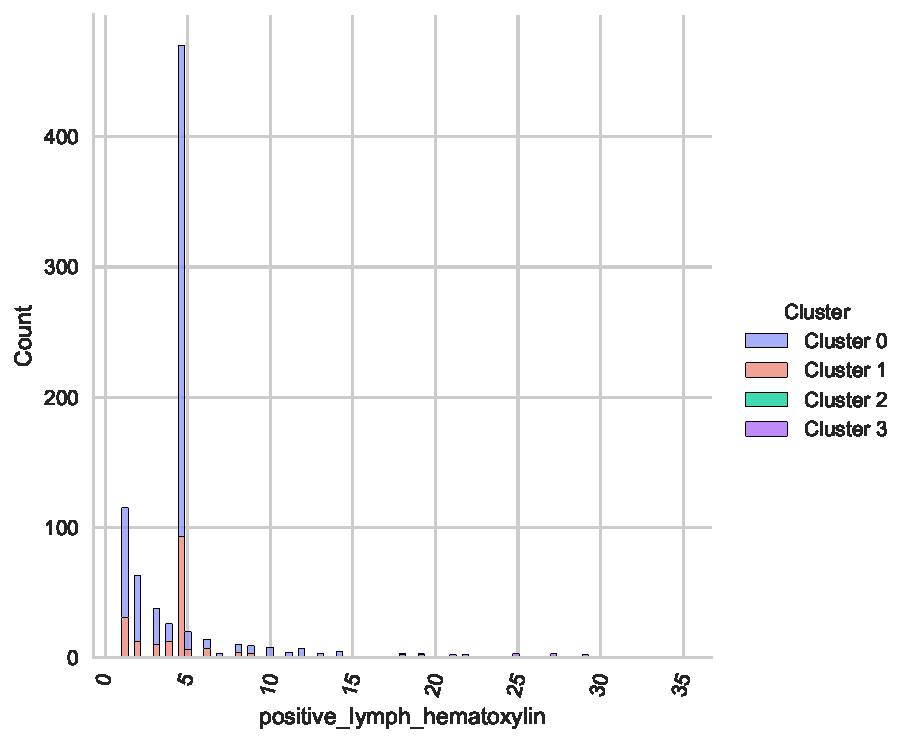
\includegraphics[width=0.22\textwidth]{NOTEBOOK/IMAGENES_BIRCH_DESCRIPTIVAS/21} 
			& 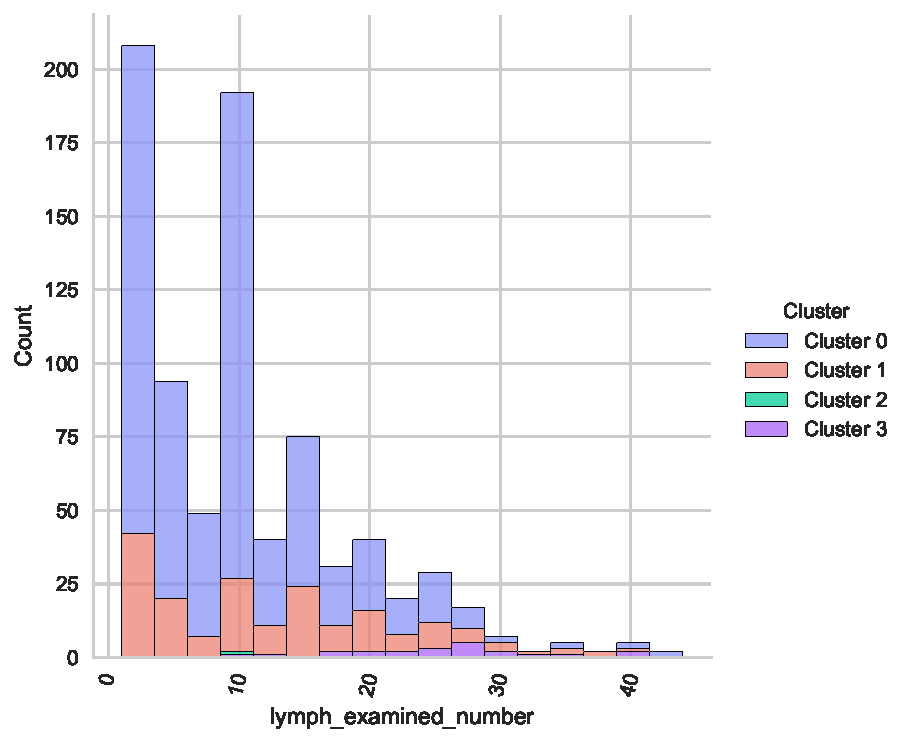
\includegraphics[width=0.22\textwidth]{NOTEBOOK/IMAGENES_BIRCH_DESCRIPTIVAS/22} 
			& 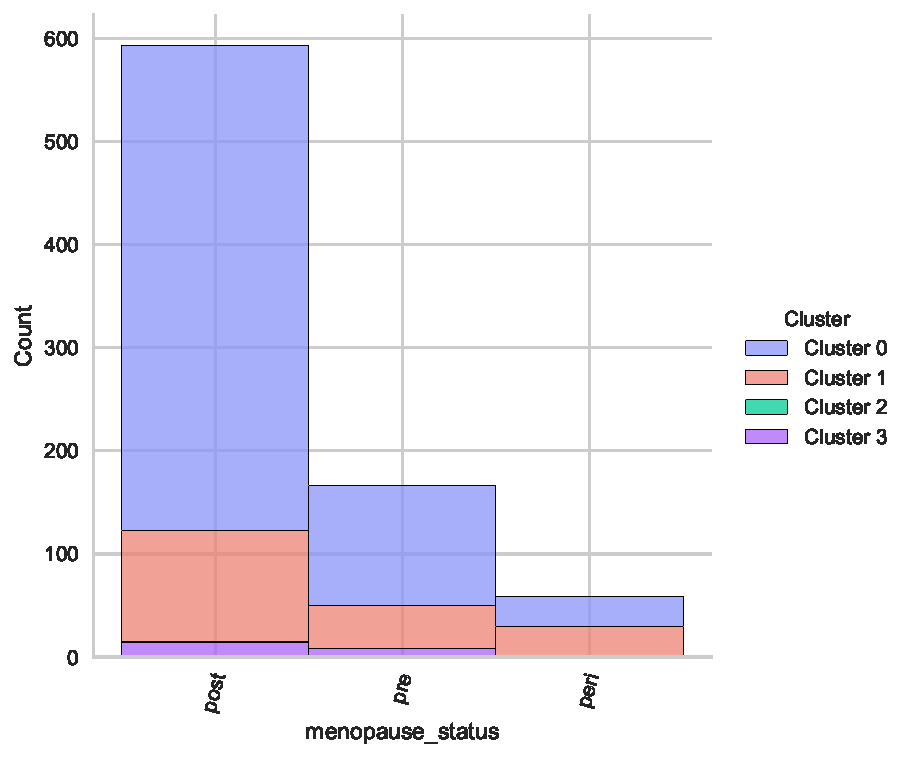
\includegraphics[width=0.22\textwidth]{NOTEBOOK/IMAGENES_BIRCH_DESCRIPTIVAS/23} 
			& 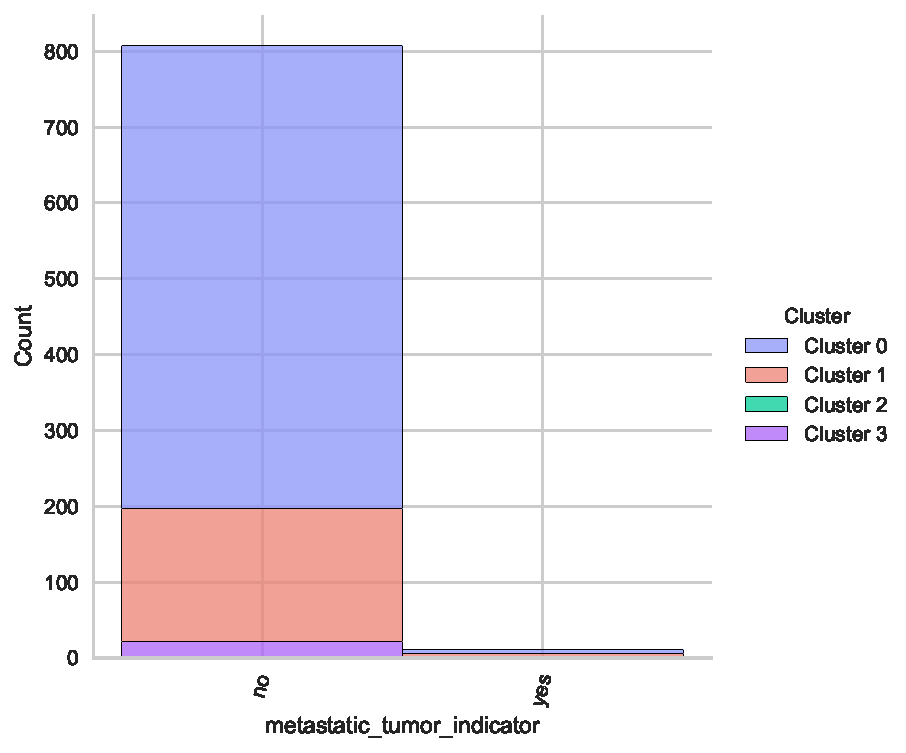
\includegraphics[width=0.22\textwidth]{NOTEBOOK/IMAGENES_BIRCH_DESCRIPTIVAS/24} 
			\\  \hline 
			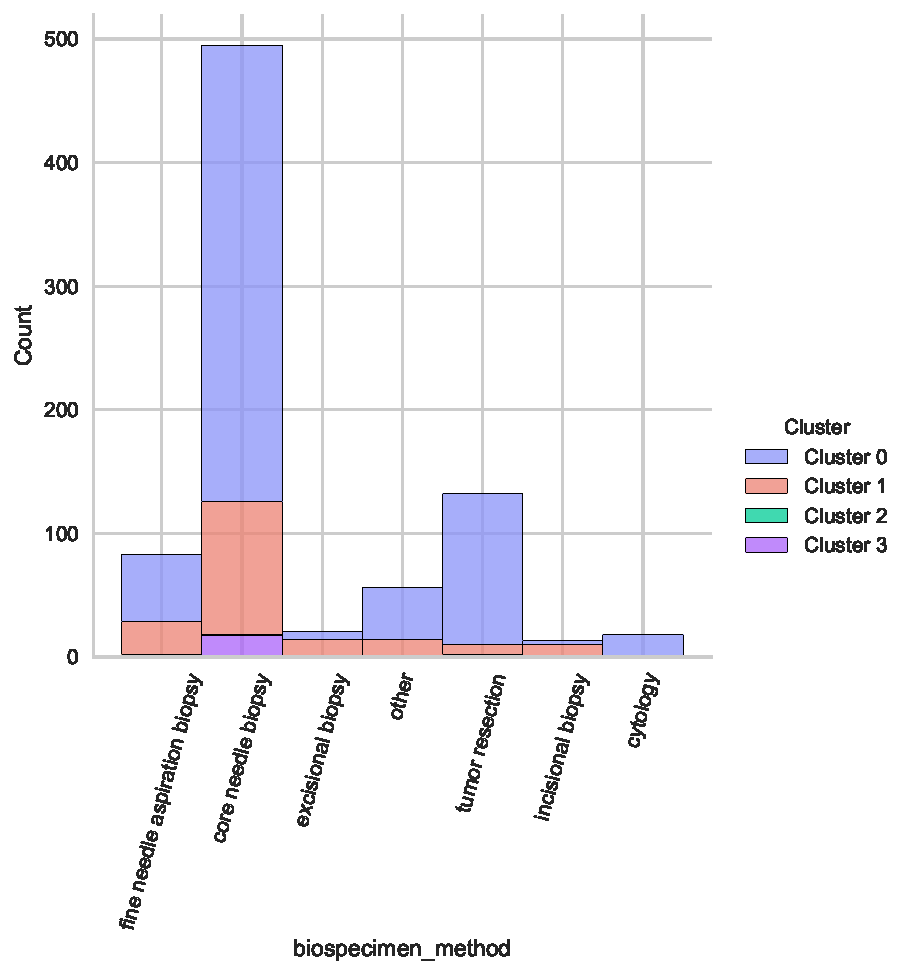
\includegraphics[width=0.22\textwidth]{NOTEBOOK/IMAGENES_BIRCH_DESCRIPTIVAS/25} 
			& 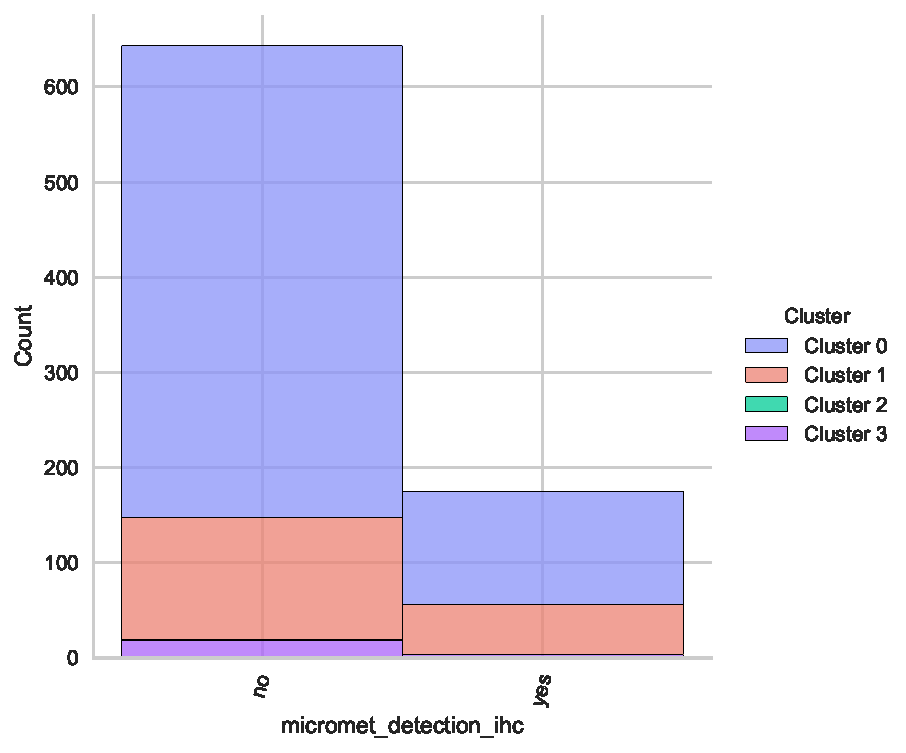
\includegraphics[width=0.22\textwidth]{NOTEBOOK/IMAGENES_BIRCH_DESCRIPTIVAS/26} 
			& 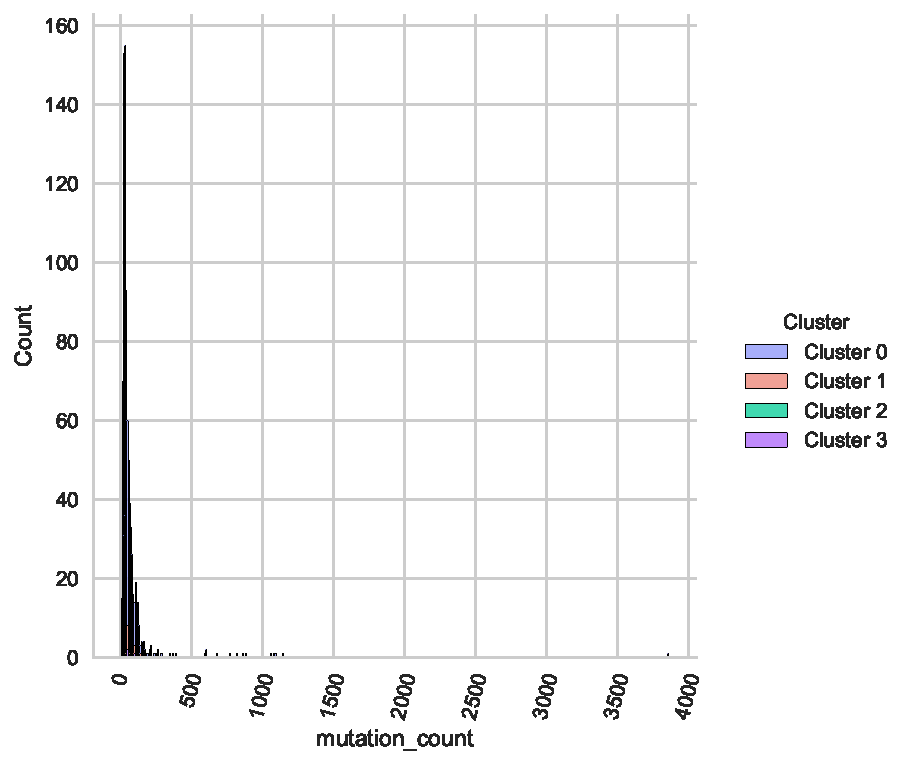
\includegraphics[width=0.22\textwidth]{NOTEBOOK/IMAGENES_BIRCH_DESCRIPTIVAS/27} 
			& 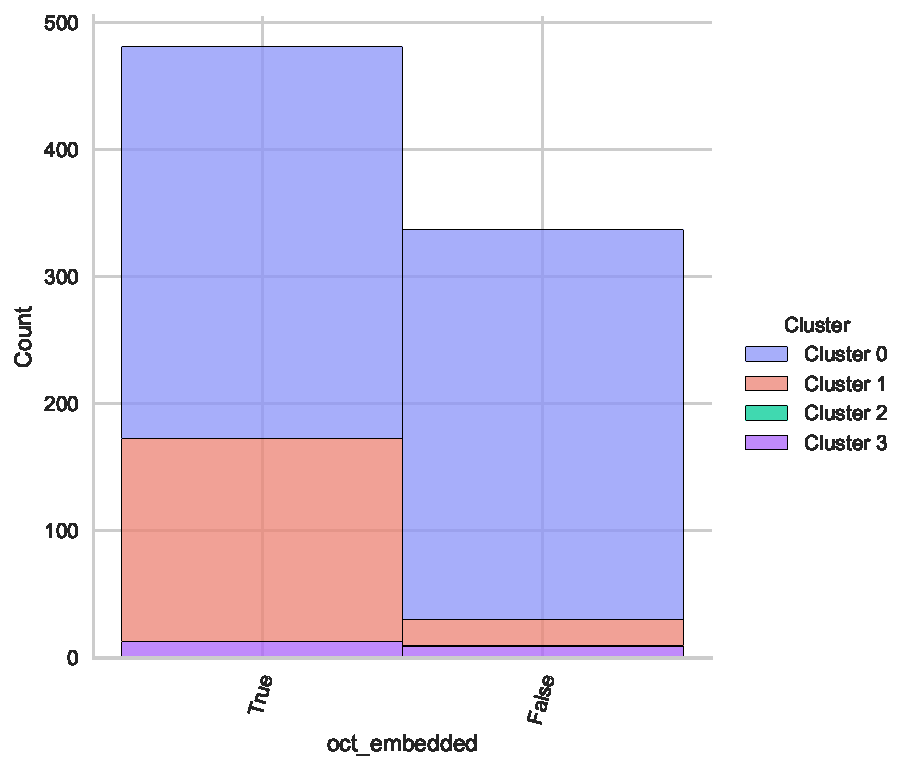
\includegraphics[width=0.22\textwidth]{NOTEBOOK/IMAGENES_BIRCH_DESCRIPTIVAS/28}
			\\  \hline 
			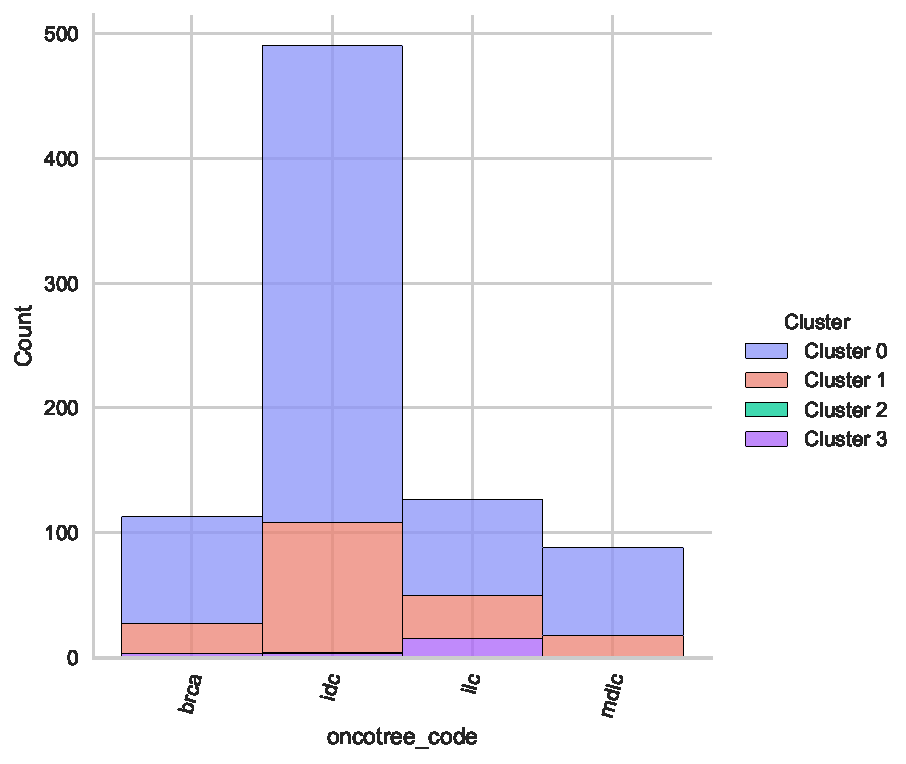
\includegraphics[width=0.22\textwidth]{NOTEBOOK/IMAGENES_BIRCH_DESCRIPTIVAS/29} 
			& 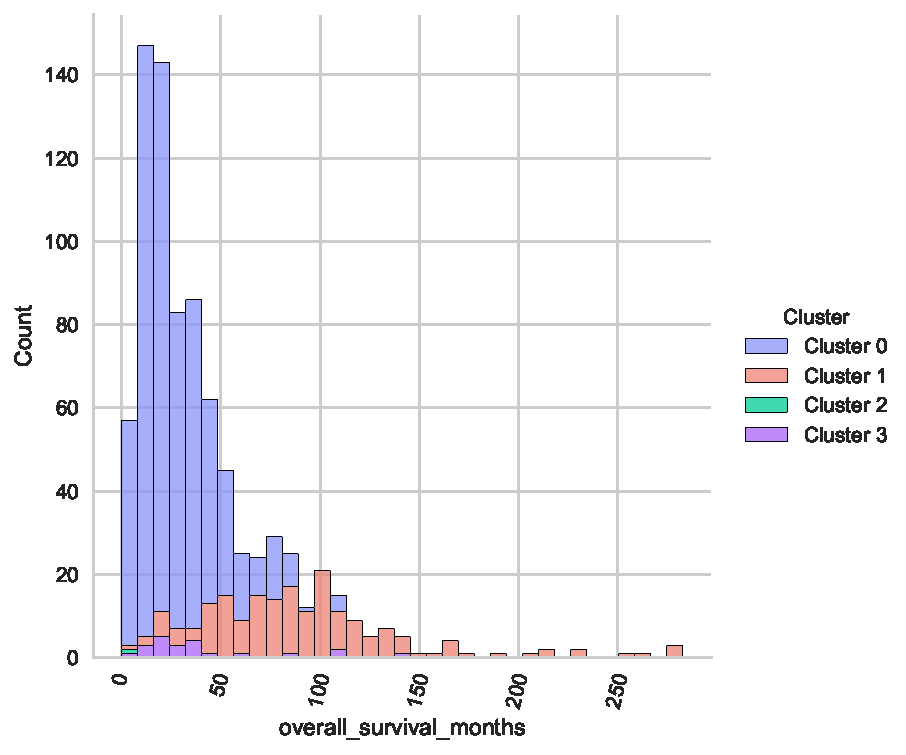
\includegraphics[width=0.22\textwidth]{NOTEBOOK/IMAGENES_BIRCH_DESCRIPTIVAS/30} 
			& 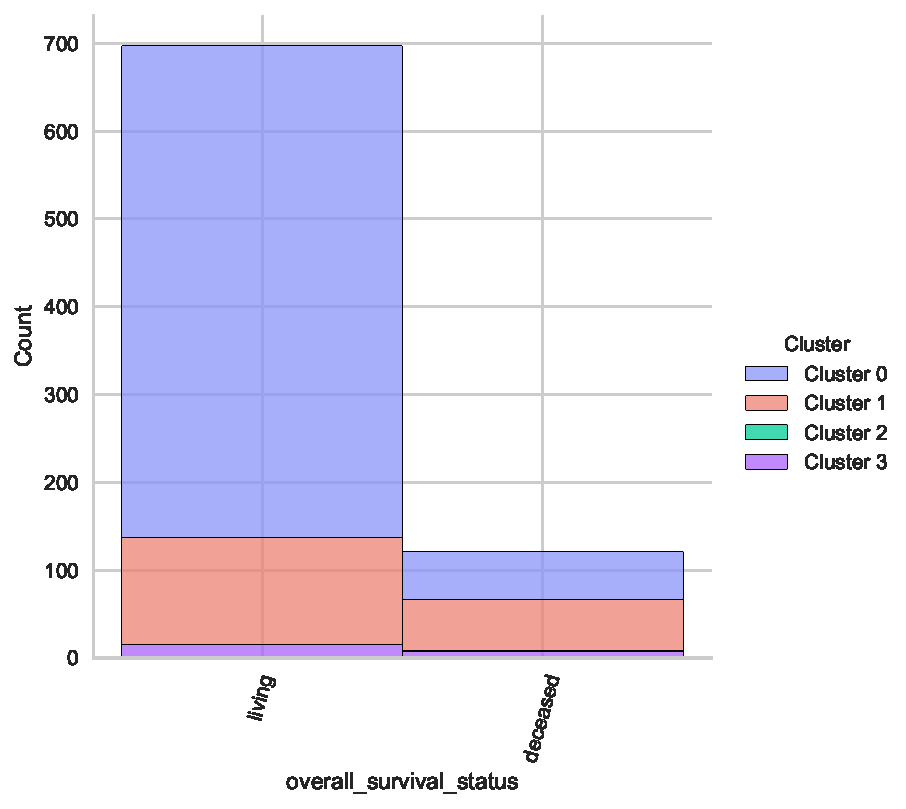
\includegraphics[width=0.22\textwidth]{NOTEBOOK/IMAGENES_BIRCH_DESCRIPTIVAS/31} 
			& 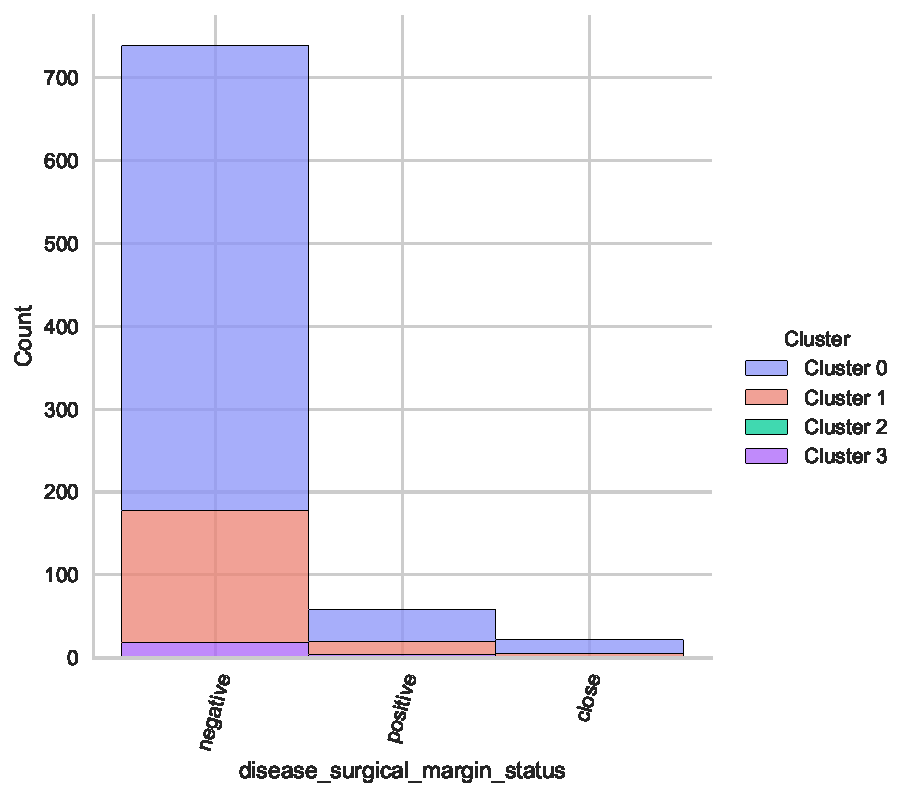
\includegraphics[width=0.22\textwidth]{NOTEBOOK/IMAGENES_BIRCH_DESCRIPTIVAS/32}
			\\  \hline 
			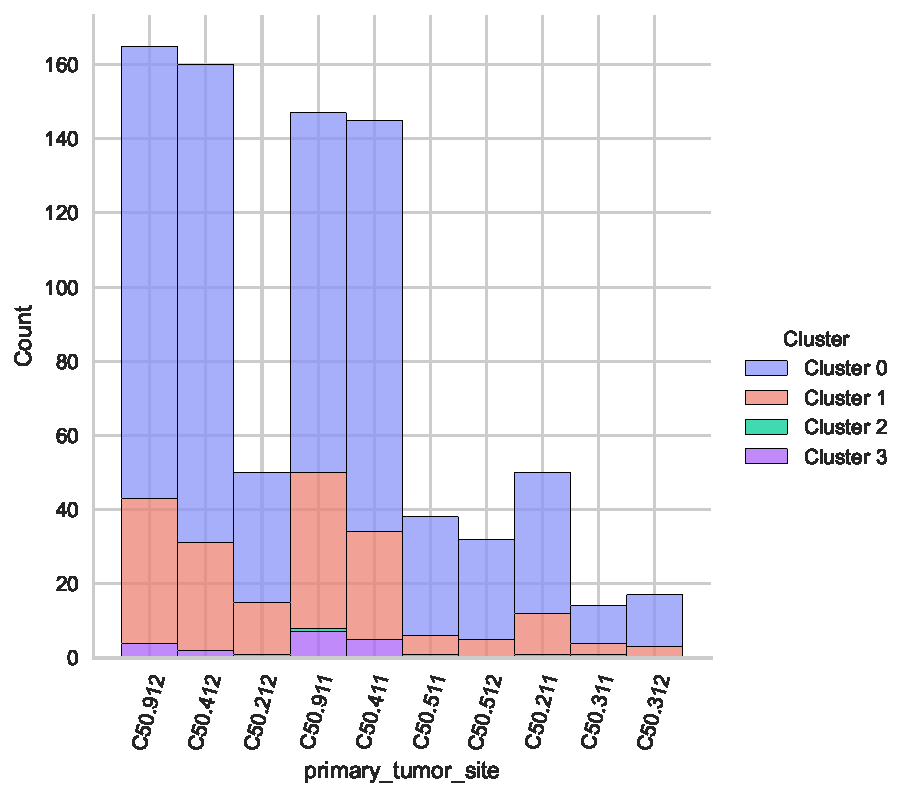
\includegraphics[width=0.22\textwidth]{NOTEBOOK/IMAGENES_BIRCH_DESCRIPTIVAS/33} 
			& 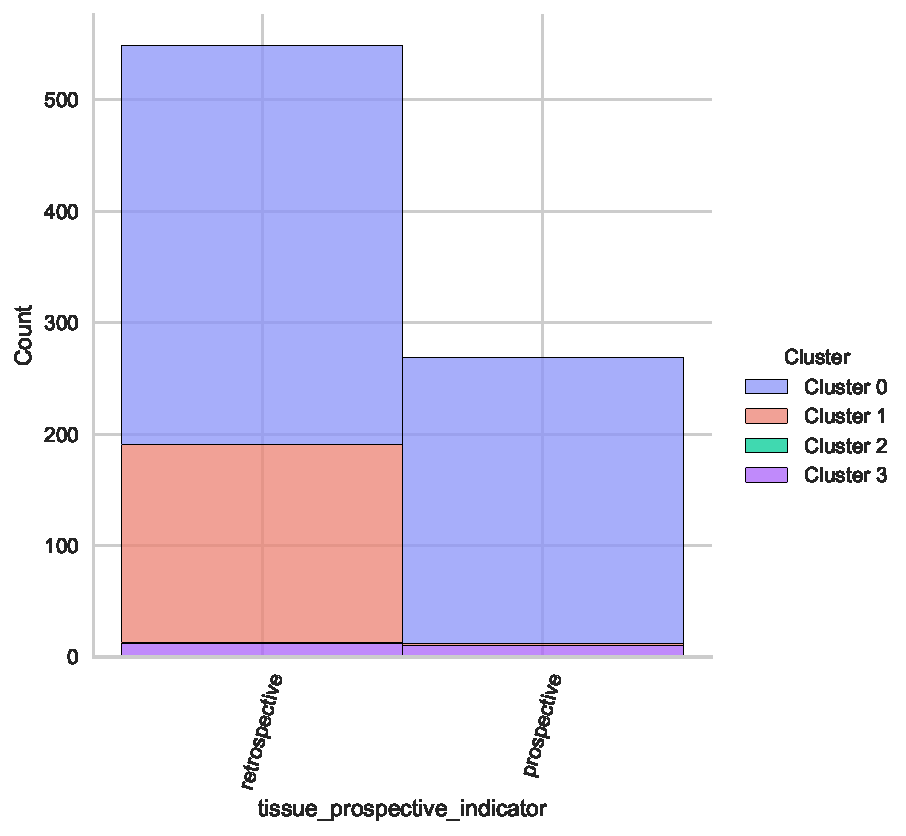
\includegraphics[width=0.22\textwidth]{NOTEBOOK/IMAGENES_BIRCH_DESCRIPTIVAS/34} 
			& 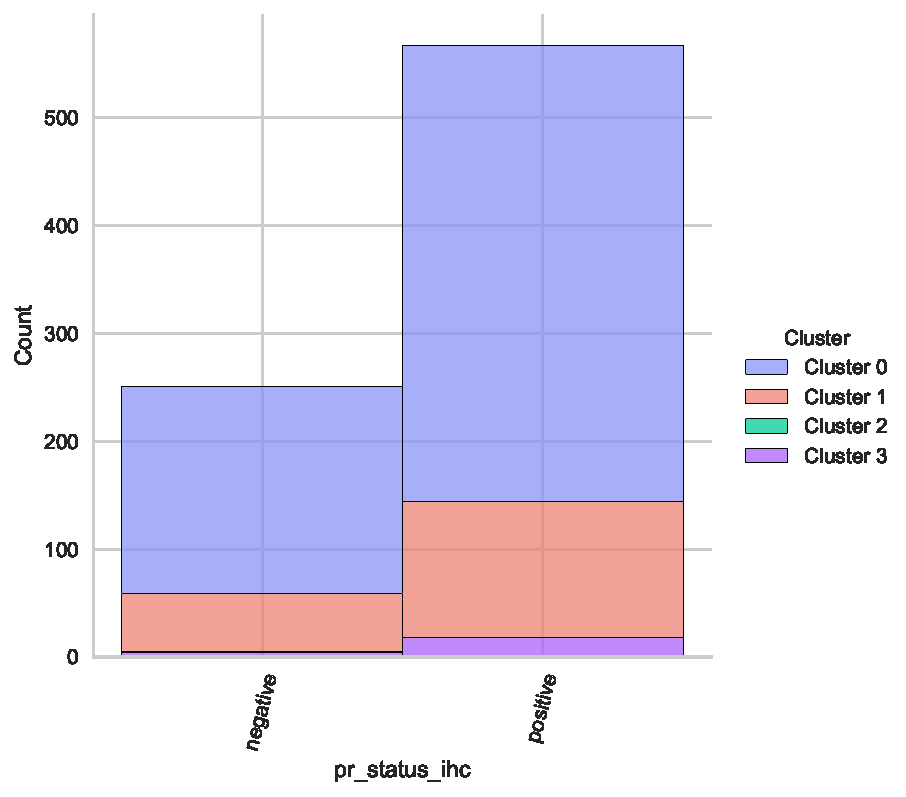
\includegraphics[width=0.22\textwidth]{NOTEBOOK/IMAGENES_BIRCH_DESCRIPTIVAS/35} 
			& 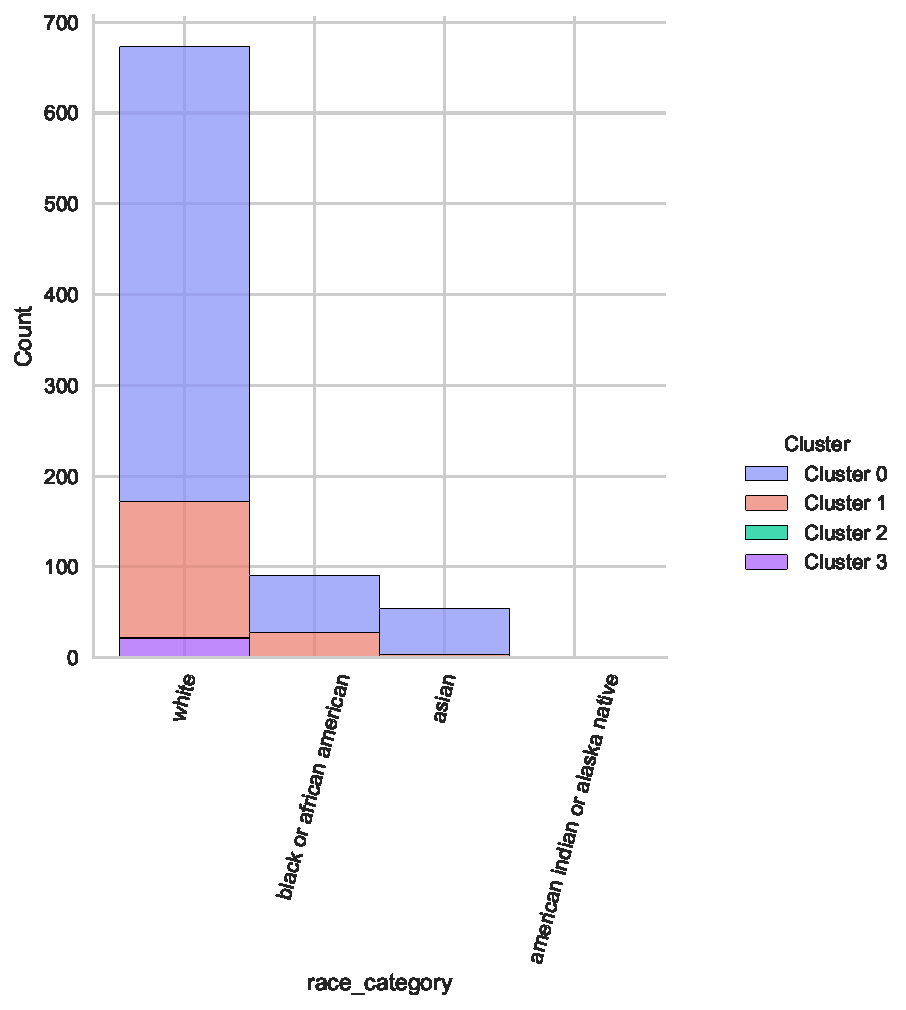
\includegraphics[width=0.22\textwidth]{NOTEBOOK/IMAGENES_BIRCH_DESCRIPTIVAS/36}         
			\\  \hline
			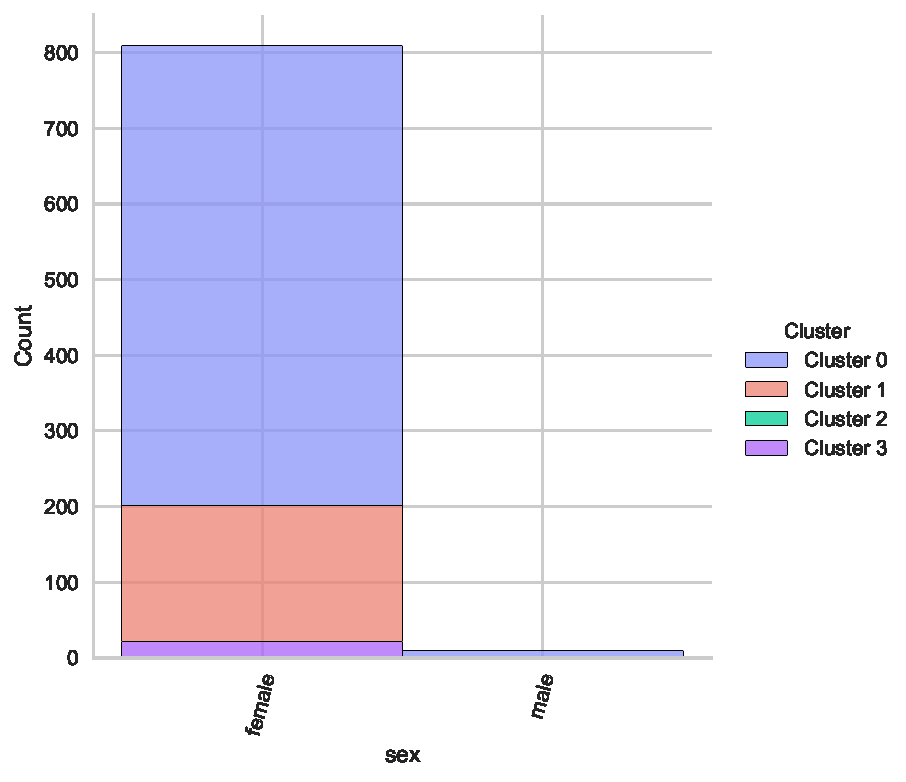
\includegraphics[width=0.22\textwidth]{NOTEBOOK/IMAGENES_BIRCH_DESCRIPTIVAS/37} 
			& 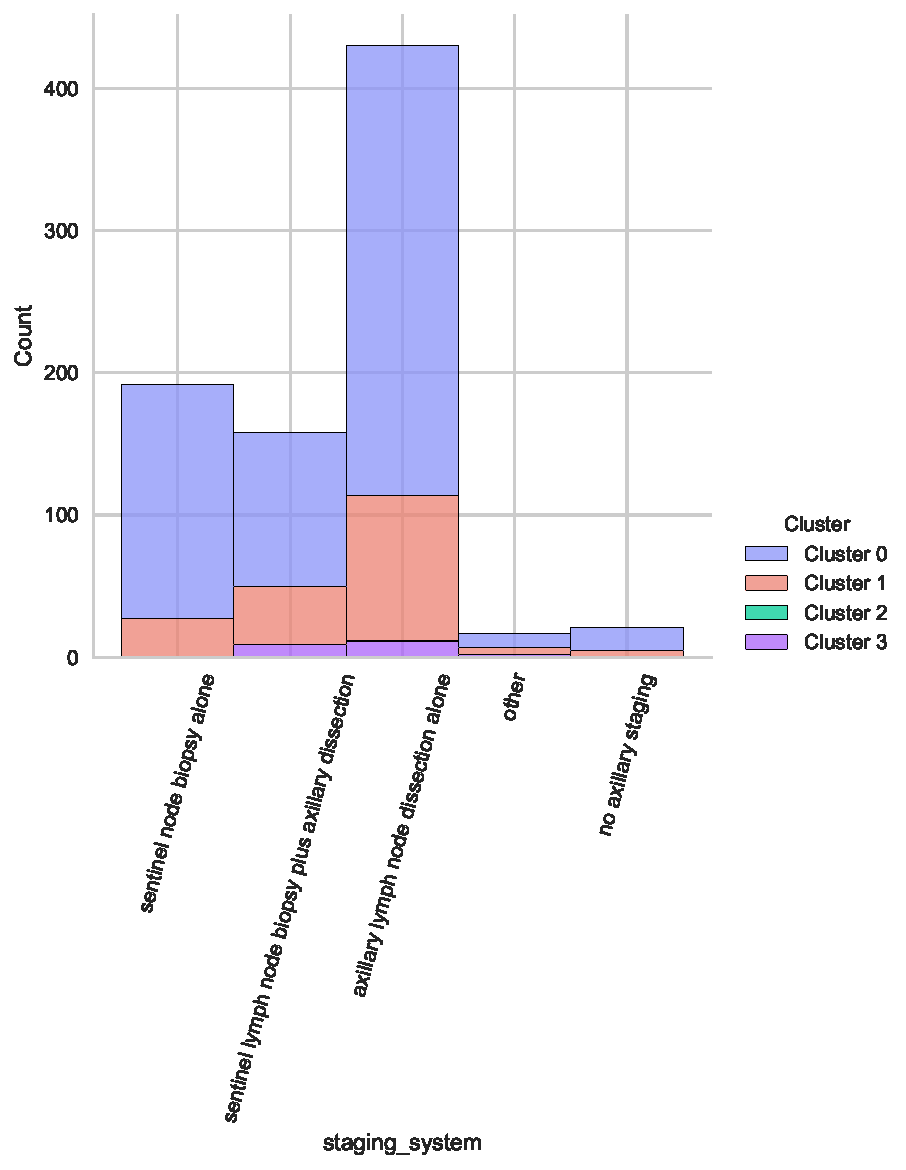
\includegraphics[width=0.22\textwidth]{NOTEBOOK/IMAGENES_BIRCH_DESCRIPTIVAS/38} 
			& 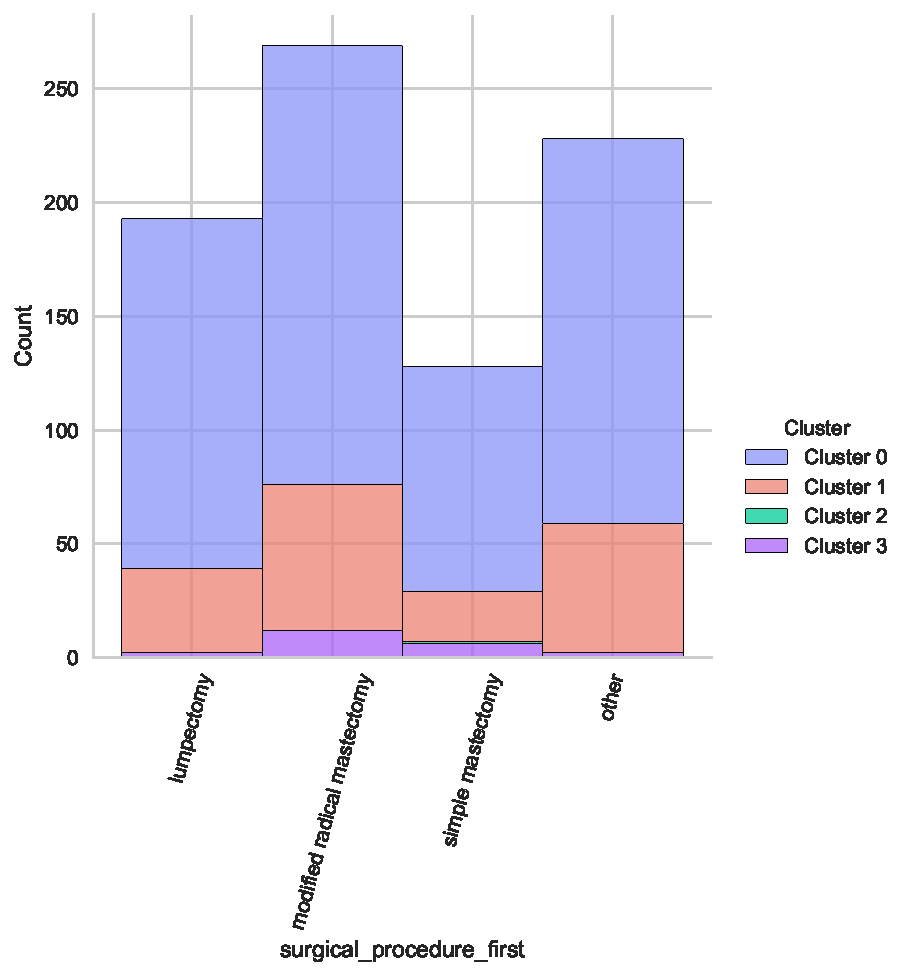
\includegraphics[width=0.22\textwidth]{NOTEBOOK/IMAGENES_BIRCH_DESCRIPTIVAS/39} 
			& 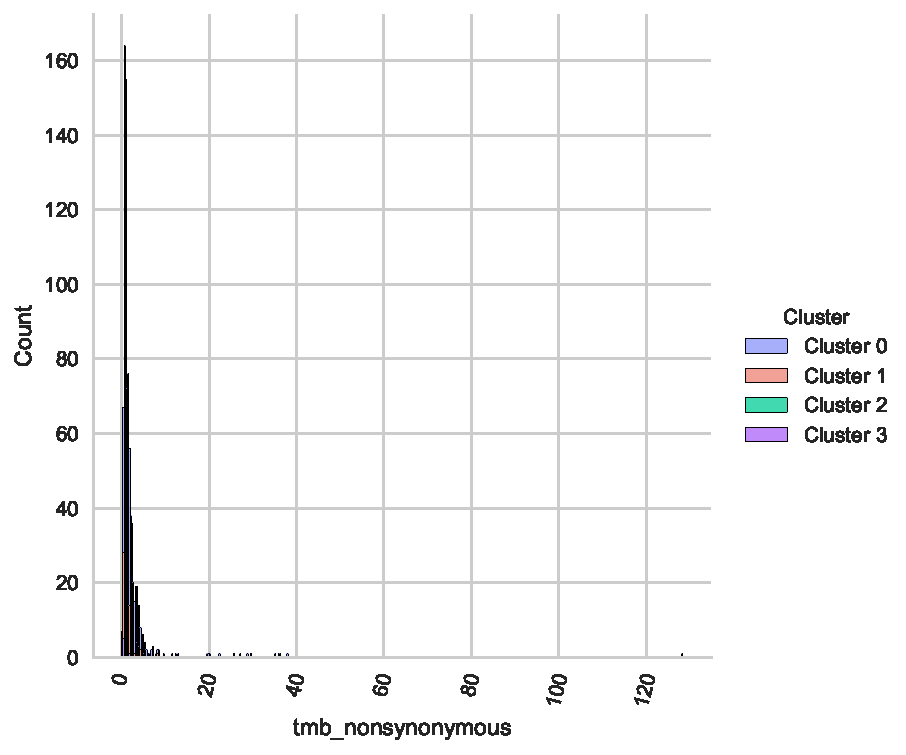
\includegraphics[width=0.22\textwidth]{NOTEBOOK/IMAGENES_BIRCH_DESCRIPTIVAS/40} 
			\\  \hline                  
		\end{tabular} 
			\caption{Clusters con características genómicas de 818 pacientes.}
			\label{clusters}
	\end{center} 
\end{table}
\break
Una vez analizados los resultados obtenidos, se observa que en los \textit {Cluster 0, 1 y 2} el Carcinoma  Ductal Invasivo (IDC) es predominante en la mayoría de los pacientes, sin embargo esta tendencia cambio en el \textit{Cluster 3} en donde el Carcinoma Lobulillar Invasivo (LBC) se presento en la mayoría de los pacientes, tal y como se puede observar en la tabla \ref{carcinoma_cluster}. 
\begin{table}[!htb]
	\begin{center} 
		\begin{tabular}{ |c|c| }
			\hline 
		      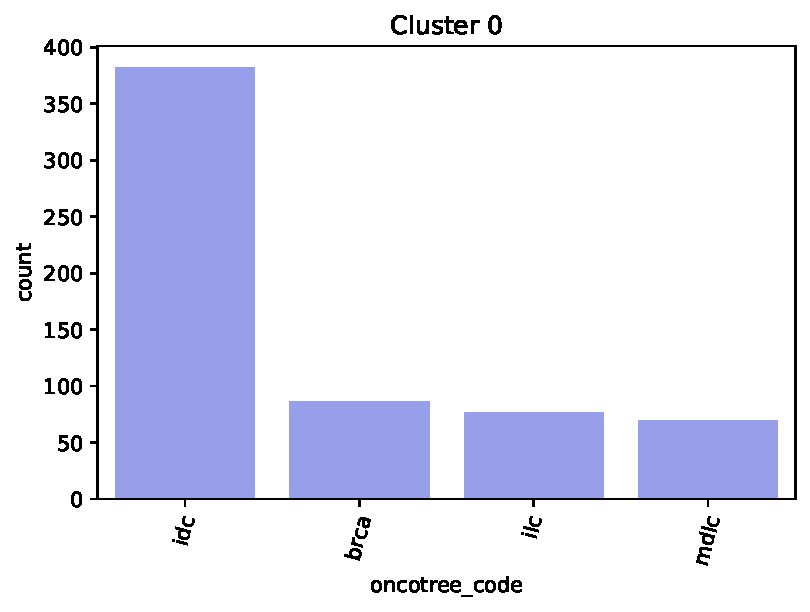
\includegraphics[width=.5\textwidth]{NOTEBOOK/IMAGENES_BIRCH_CLUSTERING/1_Cluster_0_oncotree_code} 
			& 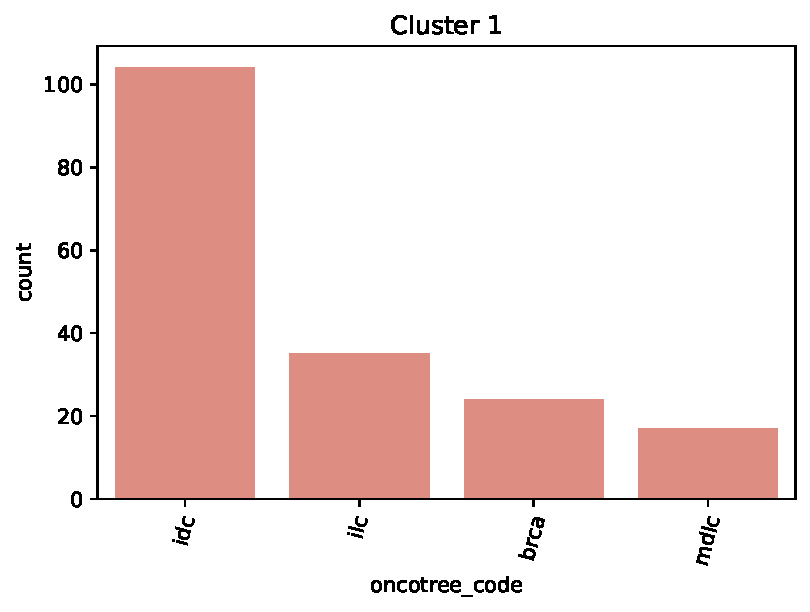
\includegraphics[width=.5\textwidth]{NOTEBOOK/IMAGENES_BIRCH_CLUSTERING/1_Cluster_1_oncotree_code} 
			\\  \hline
			  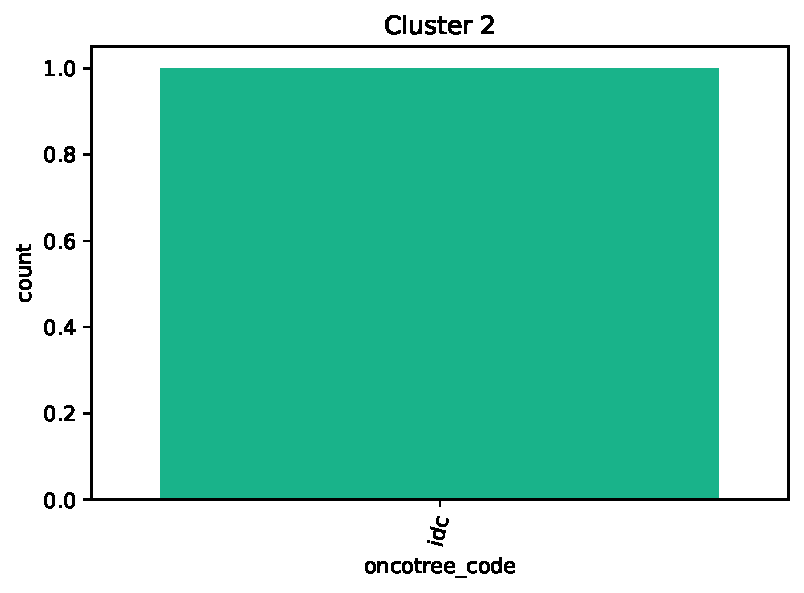
\includegraphics[width=.5\textwidth]{NOTEBOOK/IMAGENES_BIRCH_CLUSTERING/1_Cluster_2_oncotree_code} 
			& 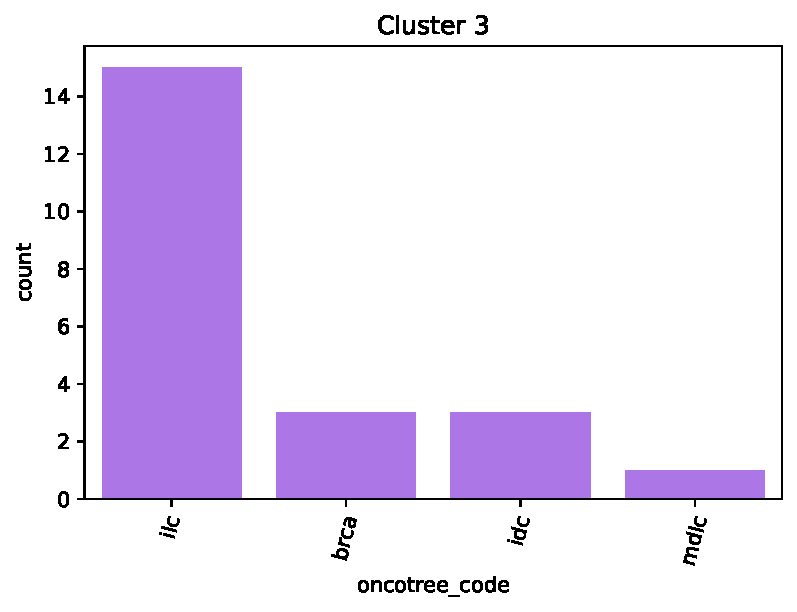
\includegraphics[width=.5\textwidth]{NOTEBOOK/IMAGENES_BIRCH_CLUSTERING/1_Cluster_3_oncotree_code} 
			\\  \hline            
		\end{tabular} 
		\caption{Clusters por tipo de carcinoma de mama.}
		\label{carcinoma_cluster}
	\end{center} 
\end{table}

Hay que mencionar que para poder determinar los atributos característicos se compararon las 41 variables de origen genómico de los 4 clusters. Se obtuvo como resultado, que 30 variables no presentaron cambio en ninguno de los clusters con respecto al análisis descriptivo realizado en las fases previas, sin embargo 11 variables presentaron diferencias en el \textit{Cluster 3} con respecto a los demás clusters, permitiéndonos identificar atributos genómicos inherentes del Carcinoma Lobulillar Invasivo (LBC) con respecto al Carcinoma Ductal Invasivo (IDC). Llegados a este punto se infiere, según el comportamiento de los datos, las siguientes apreciaciones:
\begin{table*}[htb!]
	\footnotesize
	\begin{threeparttable}
		\begin{tabular}{p{2.5cm} p{7cm} p{6.5cm}} \toprule
			\begin{center}Variable\end{center}   	 
			&\begin{center}Análisis descriptivo\end{center}             
			&\begin{center}Gráfico estadístico\end{center}\\ \hline
			%------------------------------------------------------	
			Diagnosis Age
			& La \textit{edad de diagnostico} del cáncer de mama tiene una tendencia central de 59 años, en donde la edad mínima presentada es de  26 años y la edad máxima presentada es de 90 años.
			& \begin{center}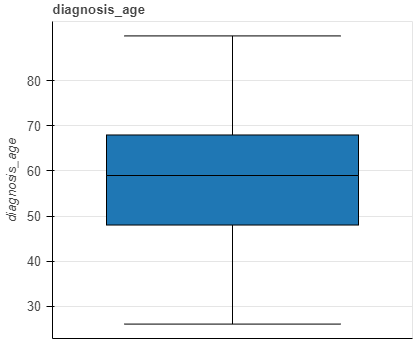
\includegraphics[width=1\linewidth]{NOTEBOOK/IMAGENES_DESCRIPTIVAS/1_diagnosis_age}\end{center}
			\\ \hline
			%------------------------------------------------------	
			AJCC Metastasis Stage Code 
			& El código AJCC para la \textit{estadificación metastásica(M) del cáncer} se visualiza en orden descendente de la siguiente manera: En primer lugar, el código \textit{m0} se presenta en 707 pacientes en donde el cáncer hizo metástasis pero no se  disemino a otras partes del cuerpo. En segundo lugar se encuentra el código \textit{mx} presentado en 96 pacientes a los cuales no fue posible medir la metástasis. En tercer lugar se encuentra el código \textit{m1} presentado en 13 pacientes en donde el cáncer se diseminó a otras partes del cuerpo. En ultimo lugar se encuentra el código \textit{cM0(i+)} presentado en 2 pacientes en los cuales no se detecto evidencia de metástasis a distancia, pero hubo un pequeño número de células en las cuales se encontró una metástasis diminuta (no mayor de 0.2 mm) detectada en ganglios linfáticos no regionales \cite{NCI}.
			& \begin{center}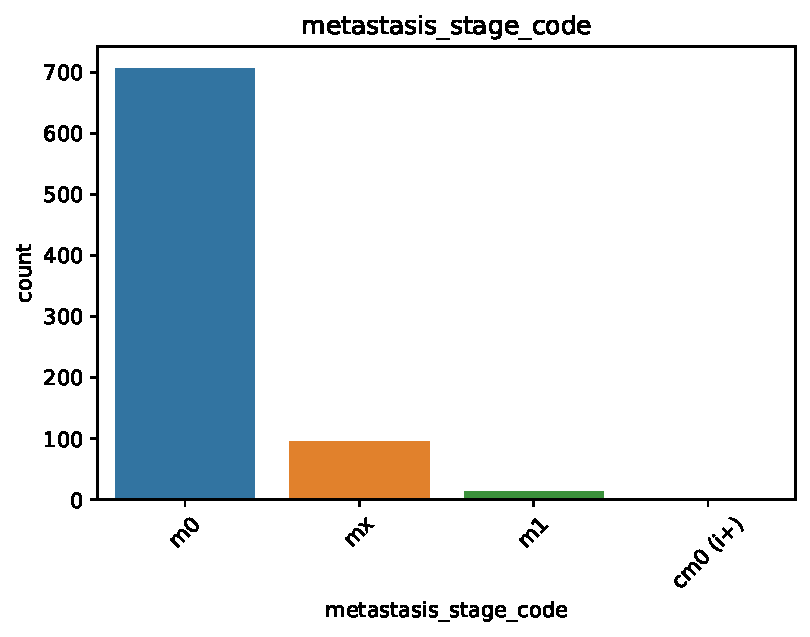
\includegraphics[width=1\linewidth]{NOTEBOOK/IMAGENES_DESCRIPTIVAS/2_metastasis_stage_code}\end{center}
			\\ \hline
		\end{tabular}
	\end{threeparttable}
\end{table*}
\clearpage


